\documentclass{article}

\usepackage{arxiv}

\usepackage[utf8]{inputenc} % allow utf-8 input
\usepackage[T1]{fontenc}    % use 8-bit T1 fonts
\usepackage{lmodern}        % https://github.com/rstudio/rticles/issues/343
\usepackage{hyperref}       % hyperlinks
\usepackage{url}            % simple URL typesetting
\usepackage{booktabs}       % professional-quality tables
\usepackage{amsfonts}       % blackboard math symbols
\usepackage{nicefrac}       % compact symbols for 1/2, etc.
\usepackage{microtype}      % microtypography
\usepackage{graphicx}

\title{Functional traits complicate the picture of temporal biodiversity
change in bird and mammal communities}

\author{
  }


% tightlist command for lists without linebreak
\providecommand{\tightlist}{%
  \setlength{\itemsep}{0pt}\setlength{\parskip}{0pt}}


% Pandoc citation processing
\newlength{\cslhangindent}
\setlength{\cslhangindent}{1.5em}
\newlength{\csllabelwidth}
\setlength{\csllabelwidth}{3em}
\newlength{\cslentryspacingunit} % times entry-spacing
\setlength{\cslentryspacingunit}{\parskip}
% for Pandoc 2.8 to 2.10.1
\newenvironment{cslreferences}%
  {}%
  {\par}
% For Pandoc 2.11+
\newenvironment{CSLReferences}[2] % #1 hanging-ident, #2 entry spacing
 {% don't indent paragraphs
  \setlength{\parindent}{0pt}
  % turn on hanging indent if param 1 is 1
  \ifodd #1
  \let\oldpar\par
  \def\par{\hangindent=\cslhangindent\oldpar}
  \fi
  % set entry spacing
  \setlength{\parskip}{#2\cslentryspacingunit}
 }%
 {}
\usepackage{calc}
\newcommand{\CSLBlock}[1]{#1\hfill\break}
\newcommand{\CSLLeftMargin}[1]{\parbox[t]{\csllabelwidth}{#1}}
\newcommand{\CSLRightInline}[1]{\parbox[t]{\linewidth - \csllabelwidth}{#1}\break}
\newcommand{\CSLIndent}[1]{\hspace{\cslhangindent}#1}

\usepackage{lineno}
\linenumbers
\usepackage{booktabs}
\usepackage{longtable}
\usepackage{array}
\usepackage{multirow}
\usepackage{wrapfig}
\usepackage{float}
\usepackage{colortbl}
\usepackage{pdflscape}
\usepackage{tabu}
\usepackage{threeparttable}
\usepackage{threeparttablex}
\usepackage[normalem]{ulem}
\usepackage{makecell}
\usepackage{xcolor}
\begin{document}
\maketitle


\begin{abstract}
Aim: Despite unprecedented environmental change due to anthropogenic
pressure, recent work has found increasing dissimilarity due to turnover
but no overall trend in species diversity through time at the local
scale. Functional diversity provides a potentially powerful alternative
approach for understanding community composition by linking shifts in
species identity to the characteristics that confer ecosystem processes.
Here we present the first multi-taxa, multi-system analysis of
functional change through time.

Location: Global, with a North American focus

Time period: 1923-2014

Major taxa studied: Mammals, Birds

Methods: We paired thousands of bird and mammal assemblage time series
from the BioTIME database with existing trait data representative of a
species' functional role to reconstruct time series of functional
diversity and composition metrics. Using generalized linear mixed
models, we estimated general trends in those metrics and trends for
individual studies.

Results: We found evidence of decreasing functional richeness for mammal
communities and increasing functional evenness in marine communities,
but otherwise no overall trends in functional diversity metrics, which
held even after correcting for changes in species richness. With the
exception of those two trends, study characteristics such as taxa,
realm, biome, or protection status did not distinguish between types of
change exhibited by communities. At the study-level, there was
substantial heterogeneity in the direction and type of functional change
exhibited. We further did not find evidence to support multiple
predictions for inidividual traits, including decreasing body size,
dietary shifts, or changes in foraging strata.

Main Conclusions: General trends indicate that on the aggregate one type
of functional shift is not more prevalant than the other across many
taxa, biomes, and realms. Loss of functional richness in mammal
communities indicates that they are on average faring worse than bird
communities. At the study-level, the majority group of studies showed no
species or functional trends, but other types of change were found for
multiple studies, including studies experiencing changes in functional
redundancy, increased species and functional richness, or loss of
functional richness. With no one prevailing scenario of change, it will
be critical to link change scenarios to ecological context.
\end{abstract}

\keywords{
    biodiversity change
   \and
    functional traits
   \and
    global change
   \and
    time series
  }

\hypertarget{introduction}{%
\section{Introduction}\label{introduction}}

Ecological communities are experiencing unprecedented change as a result
of anthropogenic pressures such as climate change, land use change, and
invasive species. Impacts of these pressures are well documented at a
global scale by an accelerating global extinction rate (1), and
fundamental changes in some of the most well-studied systems (e.g.~coral
bleaching, 2). At the local scale however, species diversity tells a
different story. Recent syntheses of local trends in biodiversity over
time have found no net change in local species diversity despite ongoing
turnover (3--6) and evidence of significant shifts in community
composition underlying consistent species richness (7--9). While
communities are clearly changing, our most common species-based
approaches do not fully capture the nature of that change.

\textcolor{blue}{Using general trends derived from limited data as a diagnostic for the state of biodiversity or directing conservation action is a topic of ongoing debate.}
Global analyses have been heavily criticized for geographic biases, lack
of data in the most heavily impacted areas, and exclusion of individual
studies' ecological context (10--12). Many of these criticisms reflect
limitations of ecological data on the whole,
\textcolor{blue}{leading to a call for additional data not only to fill geographic and temporal gaps, but to flesh out key characteristics of communities}
(13, 14).

Functional diversity offers a potentially powerful addition to
species-based approaches for detecting and describing community change
by providing a mechanistic link between species' response to
environmental change (\emph{response traits}) and the processes they
perform (\emph{effect traits}) (15--17). By describing the functional
trait space, functional diversity metrics capture the disproportionate
impact of losses or gains of functionally unique species. Functional
diversity metrics
\textcolor{blue}{may therefore illuminate joint responses from functionally similar species or communities undetectible by looking at species identity alone.}

\textcolor{blue}{The expectation for functional diversity change across communities is not obvious from past work, and may or may not follow taxonomic trends}
(13). While \textcolor{blue}{loss of functional diversity} is frequently
cited as one of the most pressing concerns of the anthropocene (18--20),
\textcolor{blue}{functional diversity may be maintained even when species are lost from a community}
(21, 22). Forecasts of functional loss range from negligible (23) to
dire (24, 25). And while some observed trends show significant
functional loss (26) others document no loss even in some of the most
heavily impacted communities (27--29). On paleoecological time scales,
\textcolor{blue}{the functional space} shows mixed responses to
environmental change and extinction events (30, 31), with significant
impacts of species extinctions on functional diversity in some taxa and
not others (32). For some time periods, functional diversity appears to
be maintained for substantial portions of geological time (33).
\textcolor{blue}{Contemporary, broad-scale examinations of functional change are limited to only a few taxa-focused studies, but show for example functional richness increases for both North American birds}
(34, 35) \textcolor{blue}{and ray-finned fishes, sharks, and rays} (36).

\textcolor{blue}{We have stronger expectations for changes in the prevalence of some individual traits. For example, animal body size is expected to decrease as a result of climate change, a phenomena that has been documented in multiple taxa empirically and experimentally}
(37--41).
\textcolor{blue}{There is some evidence that this holds true for birds }(42)\textcolor{blue}{, but the picture is likely more complicated for mammals, where urbanization may actually lead to larger body sizes due to novel food sources}
(43)\textcolor{blue}{, even as megafaunal loss leads to on average smaller community body size. For dietary traits, recent work documenting insect declines (citation) points to potentially significant negative impacts on insectivorous animals}
(44--46).
\textcolor{blue}{Predicted extinctions based on species-level vulnerability point to further dietary shifts, favoring increases in invertivorous species }(47).
\textcolor{blue}{Some systems also show significant shifts in the prevalence of different kinds of foragers in birds, for example loss of arboreal foragers in agricultural systems}
(48)\textcolor{blue}{, and loss of neotropical understory foragers even in protect areas}
(49).

Here we
\textcolor{blue}{leverage ongoing efforts to assemble functional trait data and recent computational advances to}
perform the first multi-taxa, multi-realm assessment of functional
diversity and composition change through time. We focus on mammal and
bird species as
\textcolor{blue}{a subset of the world's biodiversity of particular conservation concern that is heavily impacted by anthropogenic change.}While
examining trends in plants, invertebrates, and other vertebrate species
is of equal interest, trait data for those taxa raise additional
challenges such as limited and biased species coverage (50), a lack of
accepted species-level means, and differences in the types of traits
collected. To ensure comparability across taxa in trait type and data
quality we therefore focus on mammals and birds.
\textcolor{blue}{We include body mass, dietary, foraging and other behavioral traits}
that were intentionally selected to be representative of a species'
Eltonian niche, thereby summarizing the functional role they play in the
community (51). An initial assessment of amphibian trends is included in
the supplement, but excluded from general trend assessment here due to
limited geographic coverage.

We assess thousands of mammal and bird functional diversity time series
to determine whether or not
\textcolor{blue}{the addition of functional trait data gives a clarifying picture of biodiversity change across communities. We present a few areas of change consensus across communities, and even more scenarios where functional trends are unexplained and warrant further theoretical and experimental examination. We assess functional diversity trends at three different levels: general trends across communities, trends for communities with similar characteristics (taxa, biome, realm, protection status), and trends for individual studies. We further evaluate evidence of key predictions for individual traits using trait-level compositional trends, including changes in mean body size, dietary traits, and foraging strata.}

\hypertarget{material-and-methods}{%
\section{Material and Methods}\label{material-and-methods}}

\hypertarget{data}{%
\subsection{Data}\label{data}}

We obtained mammal and bird time series from the BioTIME database, a
global repository of high-quality assemblage time series
\textcolor{blue}{collected from the literature and ongoing monitoring efforts}.
\textcolor{blue}{Data is structured such that a study encompass all data collected following consistent sampling protocols and may contain multiple time series from separate locations.}
Time series represent full assemblages rather than populations of single
species (31), and all time series include abundance of observed species.
Following best practices for the database (52), studies with multiple
sample locations were split into individual time series following a
standardized spatial scale. Scale was set by a global grid with cell
size determined based on the sample extent of studies with only a single
location (see 31 for details on how sample extents were defined), with
the area of each cell set to one standard deviation away from the mean
of the single extent locations.
\textcolor{blue}{The resulting cell size for our data was approximately 95 }km\textsuperscript{2}.
All samples from a study within a single cell were considered to be a
single time series, and species abundances were combined for all
samples.

We used trait data from the Elton Trait Database, which consists of
species-level means for traits that represent species' multifaceted role
in the community (51). Traits include: body mass, diet, nocturnality,
forest foraging strata, pelagic use. With the exception of body mass,
traits were broken down into percentage or binary use for each level of
the trait type (Table \ref{tab:traitTable}).

\begin{table}

\caption{\label{tab:traitTable}Description of the traits included in the analysis broken down by categories at data type.}
\centering
\begin{tabular}[t]{l|l|>{\raggedright\arraybackslash}p{3cm}|>{\raggedright\arraybackslash}p{3cm}}
\hline
Trait & Category & Taxa & Data Type\\
\hline
 & Invertebrate &  & \\
\cline{2-2}
 & Mammals and Birds &  & \\
\cline{2-2}
 & Reptiles &  & \\
\cline{2-2}
 & Fish &  & \\
\cline{2-2}
 & Unknown Vertebrates &  & \\
\cline{2-2}
 & Scavenging &  & \\
\cline{2-2}
 & Fruit &  & \\
\cline{2-2}
 & Nectar &  & \\
\cline{2-2}
 & Seeds &  & \\
\cline{2-2}
\multirow{-10}{*}{\raggedright\arraybackslash Diet} & Other Plant & \multirow{-10}{*}{\raggedright\arraybackslash Bird and Mammal} & \multirow{-10}{*}{\raggedright\arraybackslash percentage consumed}\\
\cline{1-4}
 & Below water surface &  & \\
\cline{2-2}
 & water surface &  & \\
\cline{2-2}
 & ground &  & \\
\cline{2-2}
 & understory &  & \\
\cline{2-2}
 & > 2m, below canopy &  & \\
\cline{2-2}
 & canopy &  & \\
\cline{2-2}
\multirow{-7}{*}{\raggedright\arraybackslash Foraging Strata} & aerial &  & \multirow{-7}{*}{\raggedright\arraybackslash percentage of use}\\
\cline{1-2}
\cline{4-4}
 & yes &  & \\
\cline{2-2}
\multirow{-2}{*}{\raggedright\arraybackslash Pelagic Specialist} & no & \multirow{-9}{*}{\raggedright\arraybackslash Bird} & \\
\cline{1-3}
 & yes &  & \\
\cline{2-2}
\multirow{-2}{*}{\raggedright\arraybackslash Nocturnal} & no & \multirow{-2}{*}{\raggedright\arraybackslash Bird and Mammal} & \\
\cline{1-3}
 & yes &  & \\
\cline{2-2}
\multirow{-2}{*}{\raggedright\arraybackslash Crepuscular} & no &  & \\
\cline{1-2}
 & yes &  & \\
\cline{2-2}
\multirow{-2}{*}{\raggedright\arraybackslash Diurnal} & no & \multirow{-4}{*}{\raggedright\arraybackslash Mammal} & \multirow{-8}{*}{\raggedright\arraybackslash binary}\\
\cline{1-4}
Body Mass & - & Bird and Mammal & continous, in grams\\
\hline
\end{tabular}
\end{table}

In order to ensure taxonomic consistency across datasets, BioTIME
species were paired with trait data based on their species identifier
from the Integrated Taxonomic Information System database (retrieved
09-15-2020 from the on-line database,
\url{https://doi.org/10.5066/F7KH0KBK}), obtained through the
\texttt{taxadb} R package (53, 54). If more than one species in the
assemblage data resolved to the same identifier, observations were
considered the same species. For trait data, traits for all species of
the same identifier were averaged. Only studies for which at least 75\%
of species had trait data were included. In order to have a sufficient
number of species to calculate functional diversity metrics, years with
fewer than 5 species observed were also excluded. Sensitivity analyses
were conducted for the trait coverage threshold and the duration of
included time series.

Many studies had a variable number of samples within years. To account
for this inconsistency in sampling effort we used sample-based
rarefaction by bootstrap resampling within years for each time series
based on the smallest number of samples in a year for that time series.

Our final dataset included 2,432 time series from 50 studies in 21
countries and 12 biomes and 6 different traits (Fig \ref{fig:taxaMap}).
Data came from both terrestrial and marine realms and five biomes
(Global, Polar/Temperate, Temperate, Temperate/Tropical, Tropical). The
earliest sample was in 1923 and the most recent was in 2014.
\textcolor{blue}{While it is not possible with this data to directly assess the level of human impact occurring for each study, we include binary protection status as a coarse indicator of impact level. However, protected areas were almost exclusively from temperate terrestrial studies (with one tropical study), so results are confounded by multiple other study characteristics.}
For a full breakdown of studies and their characteristics, see the
supplement. Our final dataset reflects many of the data biases that make
global synthesis work challenging, including geographic bias, a bias
away from areas currently under the greatest threat, and a bias towards
shorter time series. We address these shortcomings and their potential
impact on our results in the discussion.

\begin{figure}
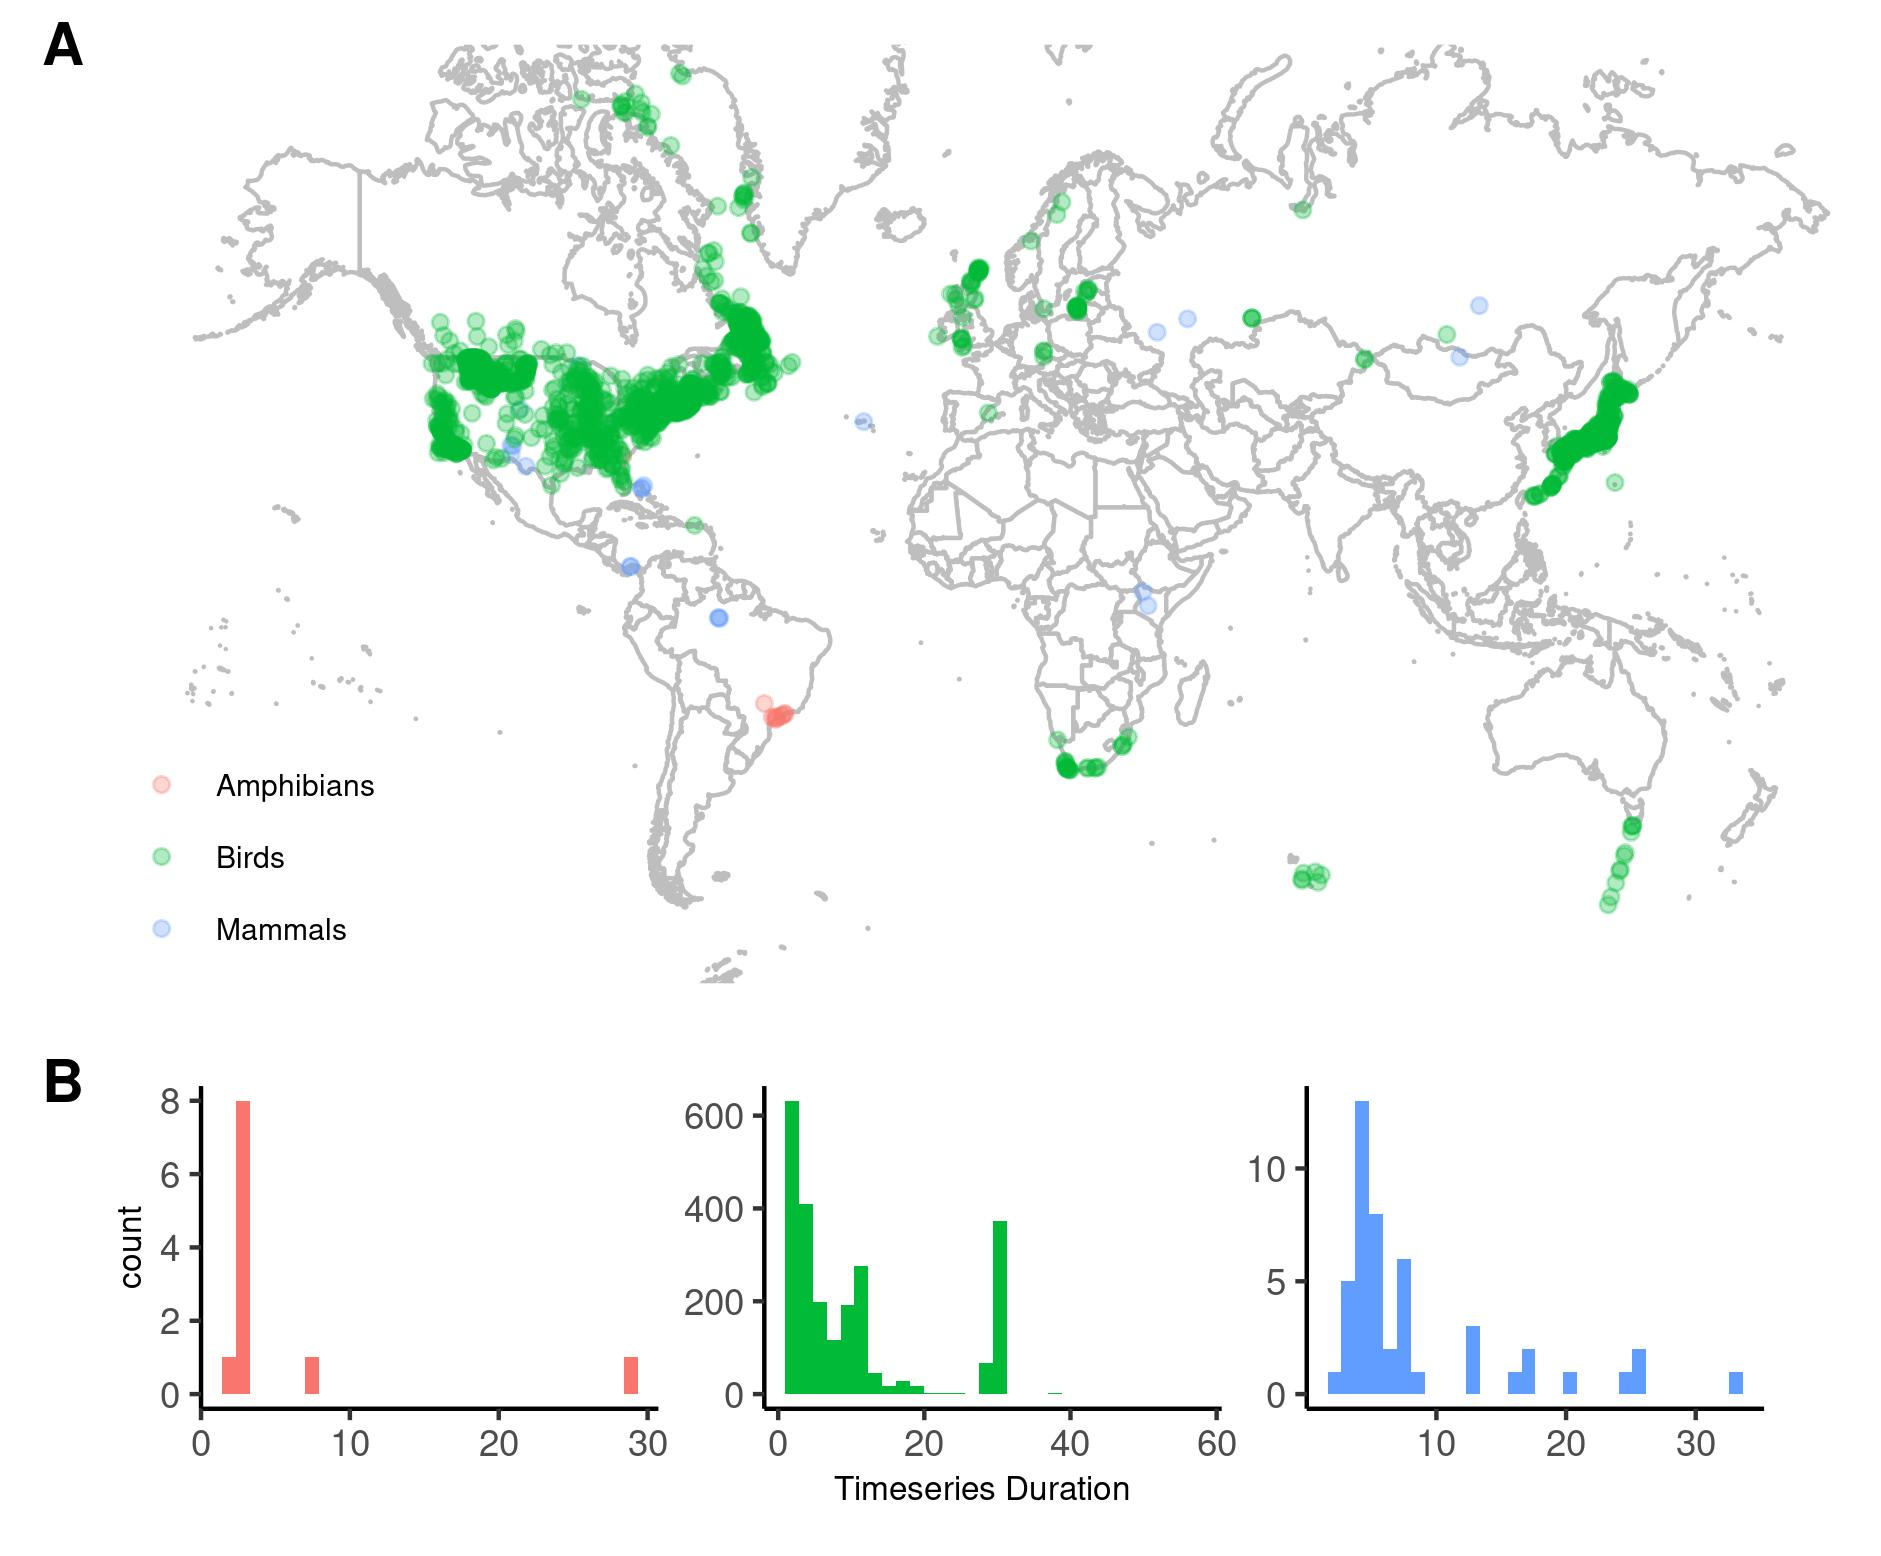
\includegraphics[width=\textwidth]{../../figures/study_map_hist} \caption{A) Map of time series locations with points colored by taxa, and B) histograms of time series duration broken down by taxa.}\label{fig:taxaMap}
\end{figure}

\hypertarget{diversity-metrics}{%
\subsection{Diversity Metrics}\label{diversity-metrics}}

We calculated yearly metrics of functional and species diversity for
each time series. Species-based metrics include species richness
(\emph{S}) and Jaccard similarity (\emph{J}) as a measure of turnover.
Jaccard similarity was calculated relative to the first observed year
for a time series. A negative trend in \emph{J} would therefore indicate
\textcolor{blue}{decreasing similiarity}. We did not impose a correction
for unobserved species as non-parametric estimators do not assign
species identities to corrected richness values, and therefore could not
be propagated to the functional diversity metrics.

Functional diversity metrics were calculated using the \emph{dbFD}
function from the \emph{FD} R package (55). Here we report functional
richness (\emph{FRic}), functional evenness (\emph{FEve}), and
functional divergence (\emph{FDiv}) which together describe three
complementary characteristics of the functional space (56, 57).
\emph{FRic} assesses the volume of the trait space occupied by species
in the community, with higher values indicating communities with species
of more extreme trait values. \emph{FEve} describes how species are
distributed across the trait space and how abundance is distributed
across species. Higher values of \emph{FEve} indicate more even spacing
of species in the trait space and individuals across species.
\emph{FDiv} measures the degree to which species and their abundances
maximize differences in the functional space. Higher values of
\emph{FDiv} therefore correspond to communities where many highly
abundant species are on the edges of the trait space.

We also calculated the community-weighted mean (\emph{CWM}) of all
continuous traits to examine \textcolor{blue}{turnover} in the
distribution of each trait.
\textcolor{blue}{Wholesale shifts in the trait space due to changes of trait means could occur even while the shape of the multidimensional trait space, as defined by functional richness, evenness, and divergence, is maintained. CWM's are therefore a way to assess whether or not turnover is occurring and what the nature of the shift may be. Hereafter we refer to results for functional metrics in two groups: functional diversity metrics (FRic, FEve, FDiv) and composition metrics (trait CWM's).}

All available trait data for each study were included in functional
diversity calculations with the exception of traits that were the same
value for all observed species in the study. For variables with multiple
levels each level was included as a separate trait axis. Continuous
traits were z-score scaled to give each trait equal weight in the trait
space (58, 59).
\textcolor{blue}{Before calculating diversity metrics, dbFD reduces the dimensionality of the trait space by performing PCoA. We limited the number of included PCoA axes to}
the maximum number of traits that fulfills the criteria \(s >= 2^t\),
where \(s\) is the number of species and \emph{t} is the number of
traits. This restriction allows for enough axes to capture the trait
space while maintaining computational feasibility (60). Metrics
incorporated weighting based on species abundance.

\hypertarget{null-models}{%
\subsection{Null Models}\label{null-models}}

To assess functional change independent of species richness we
calculated the standardized effect size (SES) for each of the three
functional diversity metrics (\emph{FRic}, \emph{FEve}, \emph{FDiv})
from null estimates (61). Null model corrections allow us to assess the
degree to which the observed functional diversity metric deviates from
the value expected by chance in a randomly assembled community. Null
estimates were calculated for each rarefied sample by randomly sampling
species from the species pool for each year and randomly assigning
observed abundances to species.
\textcolor{blue}{Species pools were unique for each time series and included all species observed over the course of sampling, therefore accounting for geographic restrictions in species availability}.
This process was repeated 500 times to get an estimate and standard
deviation of the null expectation for the metric for each rarefaction
sample for that time series. We used these values to calculate SES using
the following formula:
\(SES = [F_{obs} - mean_{(F_{null})}]/SD_{(F_{null})}\). We then
calculated the median SES estimate for each metric from all the
rarefaction samples for a time series. SES estimates can be interpreted
as how much of the functional characteristic (richness, evenness,
divergence) was observed beyond what was expected by chance for a
community of that species richness.
\textcolor{blue}{This approach will be less accurate for shorter time series, as we likley will not have captured all available species in the true species pool, but it is impossible to know whether the mean estimate from the null model is an over or under estimate without knowing the functional characteristics of the missing species.}

\hypertarget{analysis}{%
\subsection{Analysis}\label{analysis}}

We estimated general trends
\textcolor{blue}{across bird and mammals communities} for each diversity
metric using a linear mixed effects model with a random slope and
intercept for each study and each time series nested within the study,
\textcolor{blue}{methods which deal well with the inherent imbalances in our data.}
We fit 18 individual \emph{CWM} models,
\textcolor{blue}{one for each trait included in the analsysis}. All time
series with data for a given trait were included in the corresponding
\emph{CWM} model. We estimated study level trends using individual
linear models. For studies with more than one times series we fit a
random slope and intercept for time series. Some study-level models
could not be fit for five studies for at least one metric due to data
limitations, but those studies were still included in the general
models. They represented 13 of 1350 study-level models fit for each
metric. For further details see the supplement. Where appropriate,
response variables were \(log\) or \(log(x+1)\) transformed to better
fit model assumptions of residual normality.

To test for trends within and between different levels of taxa, biome,
realm, and protection status we fit separate models with each of those
factors added as a predictor interacting with time to the original model
structure. We estimated within-level slopes and calculated between-level
contrasts using the \emph{emmeans} package (v1.8.2, 62).
\textcolor{blue}{For some levels of the categorical variables we did not have a sufficient number of studies to estimate a general trend, we therefore refrained from interpreting results for levels where there were fewer than three studies.}
We assessed the impact of time series duration and start year on
study-level trends using linear models with duration and start year as
predictors. All models in our analysis were fit using the \emph{lme4}
(v1.1-30) package in R (v4.2.3) and p-values were calculated by
Satterthwaite's degrees of freedom method using the \emph{lmerTest}
(v3.1-3) package with a significance level of \(\alpha = 0.05\)
(63--65).

\hypertarget{results}{%
\section{Results}\label{results}}

We found no significant overall \textcolor{blue}{temporal} trend in
species richness or functional diversity metrics
\textcolor{blue}{including functional richness, evenness, or divergence}
(observed or \textcolor{blue}{corrected}) (Fig
\ref{fig:timeseriesPlot}). We did find a significant overall decrease in
Jaccard similarity, indicating accumulating changes in species
composition. Non-significant overall \textcolor{blue}{temporal} trends
indicate that although some studies experience increasing or decreasing
trends, the average trend across studies
\textcolor{blue}{was not significantly different from zero} (Table
\ref{tab:resultsTab}). \textcolor{blue}{Within-group} trends for
different taxa, biomes, realms, or protection statuses were also
non-significant for richness and functional diversity metrics, with the
exception of a significantly increasing trend for functional evenness of
marine studies, and a significantly decreasing functional richness slope
for mammal studies. However, trends were not exhibited for the
\textcolor{blue}{corrected} metric indicating that differences
\textcolor{blue}{in functional diversity metrics} were largely due to
changes in species richness. The general trends for \emph{CWM} models
were similarly not significant, with a significant positive trend for
only percentage of fish in diet composition.

\begin{figure}
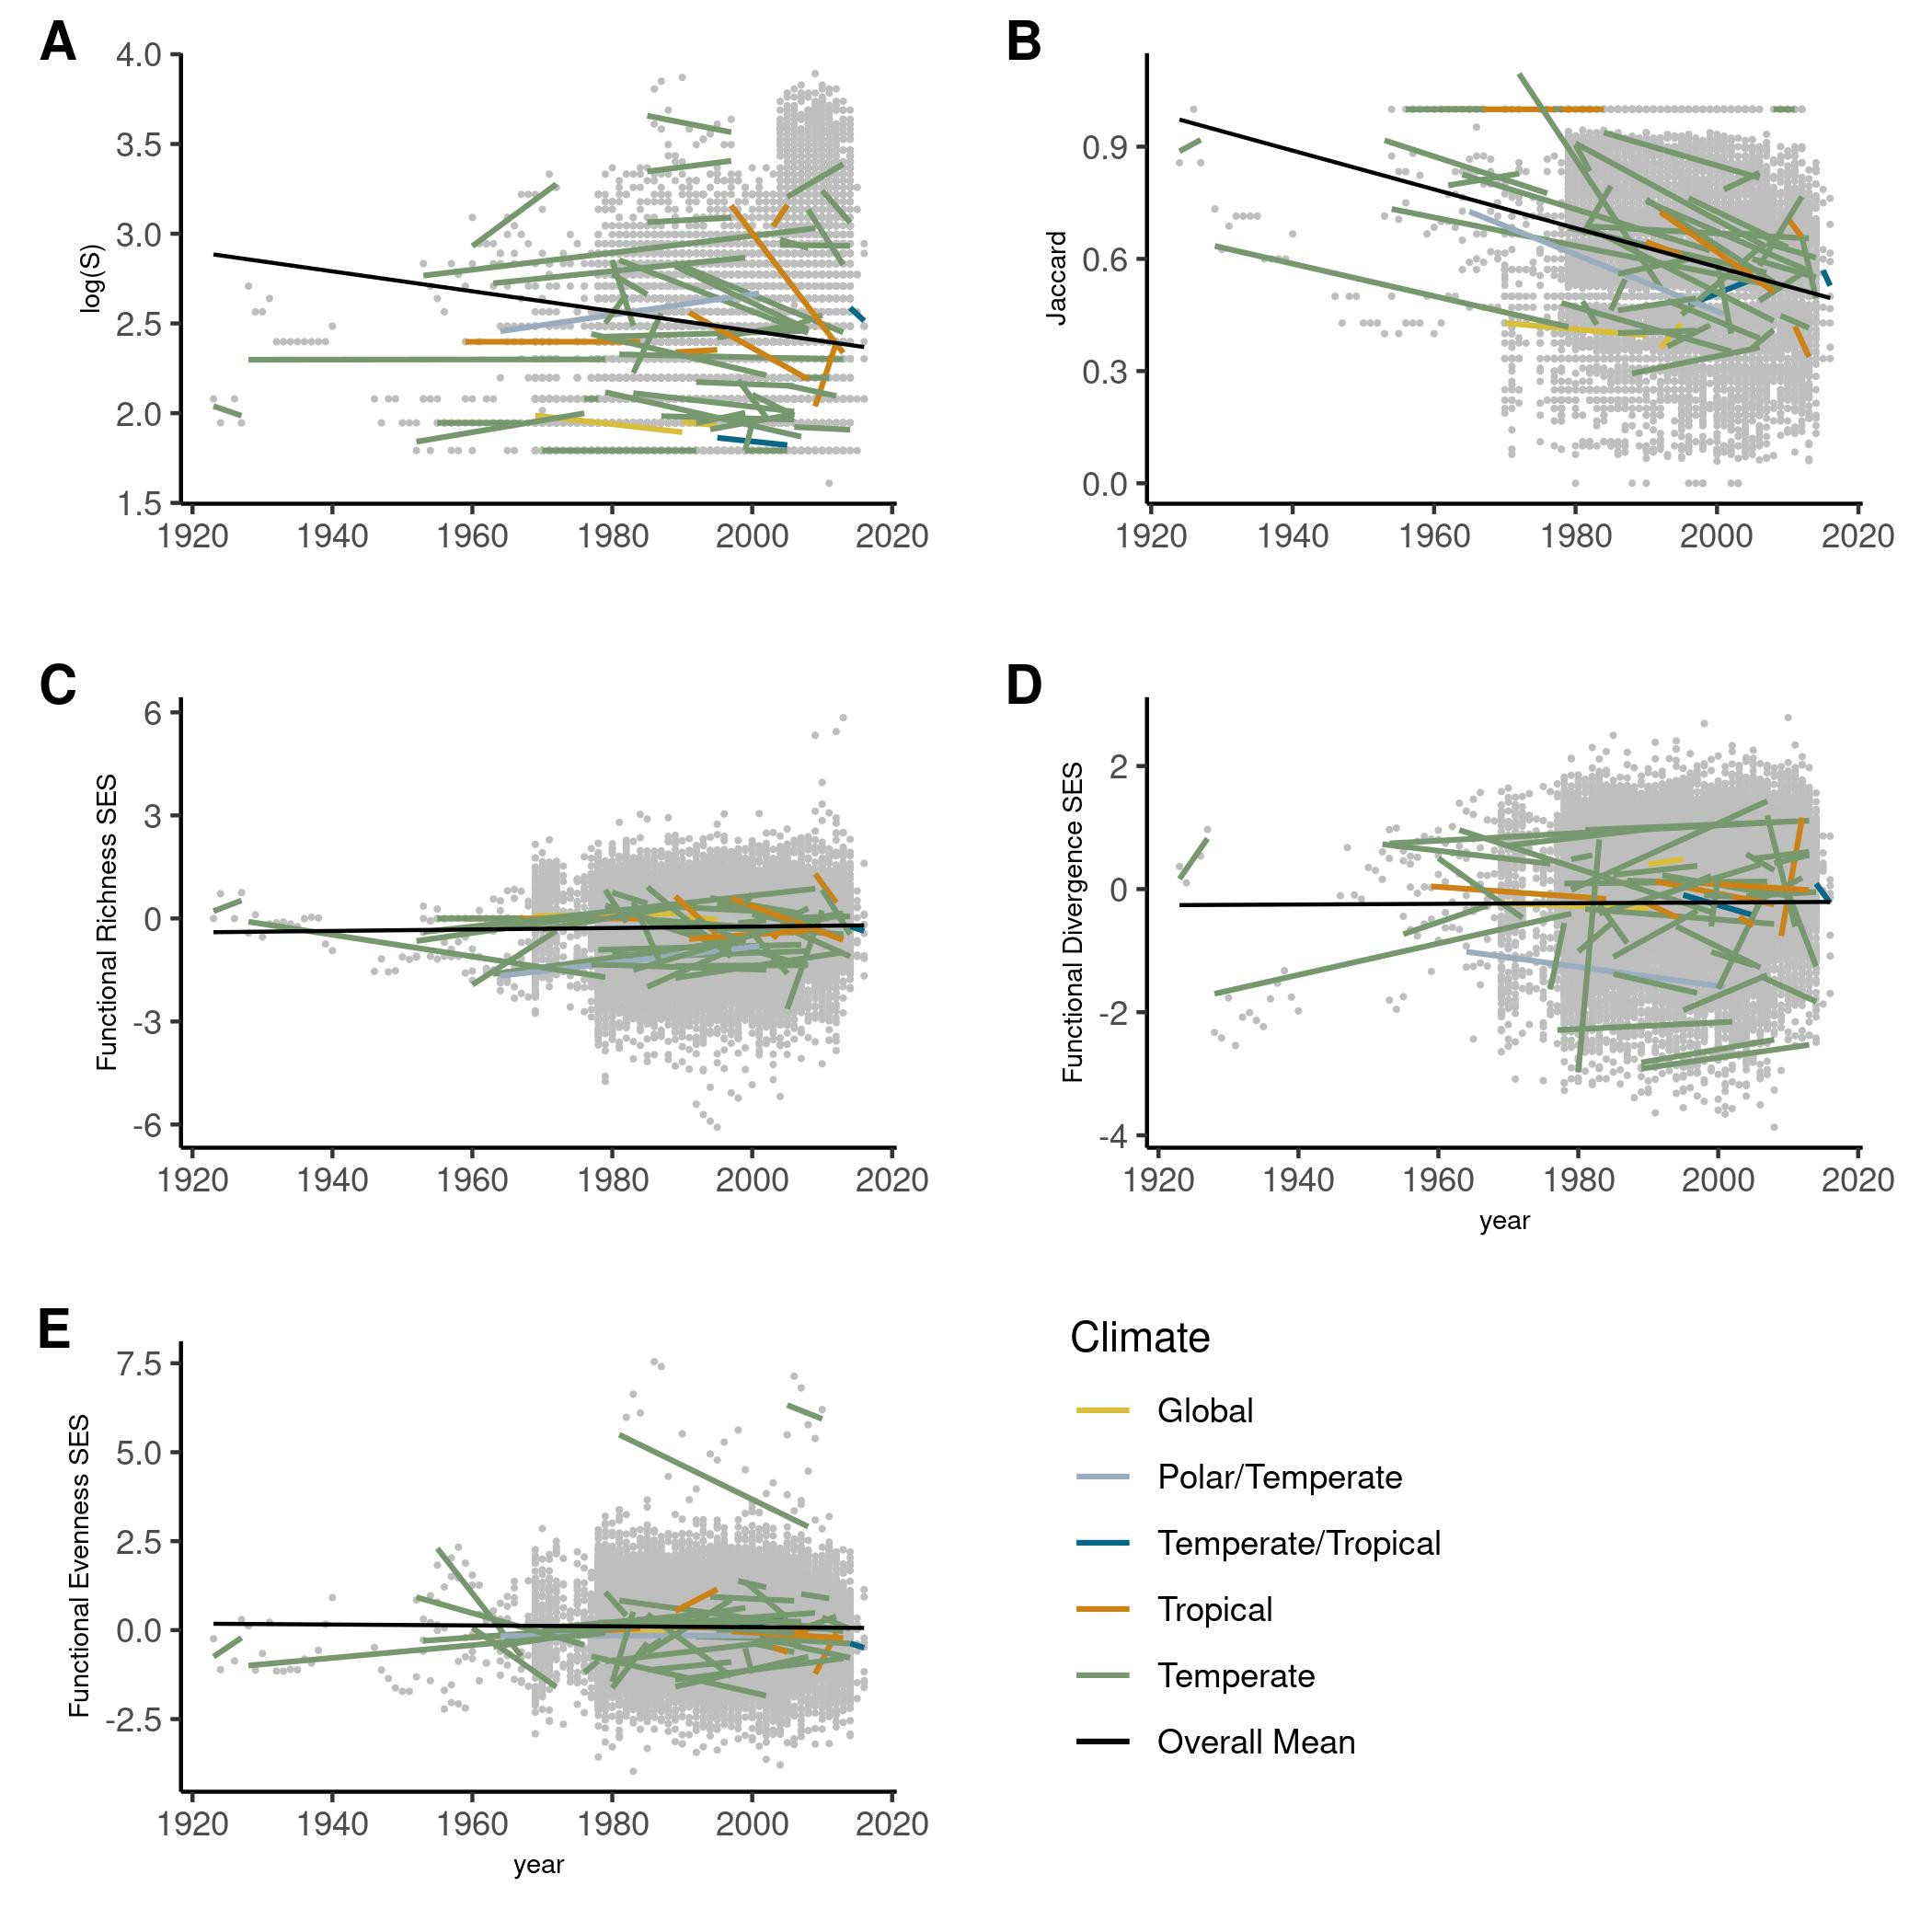
\includegraphics[width=\textwidth]{../../figures/3met_long} \caption{Plots of time series-level trends with line color corresponding to climatic region, with data points in grey and the overall mean slope for a metric in black for A) log species richness, B) Jaccard similarity, C) Functional Richness SES, D) Functional Divergence SES, and E) Functional Evenness SES}\label{fig:timeseriesPlot}
\end{figure}

\begin{table}[!h]

\caption{\label{tab:resultsTab}Model estimates and statistics for general trend models for species richness, Jaccard similarity, and corrected functional diversity metrics. Additional model estimates, including CWM models, can be found in the supplement.}
\centering
\resizebox{\linewidth}{!}{
\begin{tabular}[t]{l|l|>{\raggedright\arraybackslash}p{2cm}|l|r|r|l}
\hline
metric & effect & grouping & term & estimate & std.error & p.value\\
\hline
 &  &  & Intercept & -0.25 & 0.11 & 0.03\\
\cline{4-7}
 & \multirow{-2}{*}{\raggedright\arraybackslash fixed} & \multirow{-2}{2cm}{\raggedright\arraybackslash } & Year & 0.00 & 0.04 & 0.96\\
\cline{2-7}
 &  &  & SD Intercept & 0.60 &  & \\
\cline{4-7}
 &  &  & SD Year & 0.11 &  & \\
\cline{4-7}
 &  & \multirow{-3}{2cm}{\raggedright\arraybackslash study} & Corr(Intercept, Year) & -0.16 &  & \\
\cline{3-7}
 &  &  & SD Intercept & 0.60 &  & \\
\cline{4-7}
 &  &  & SD Year & 0.23 &  & \\
\cline{4-7}
\multirow{-8}{*}{\raggedright\arraybackslash SES\_FDiv} & \multirow{-6}{*}{\raggedright\arraybackslash random} & \multirow{-3}{2cm}{\raggedright\arraybackslash time series within study} & Corr(Intercept, Year) & -0.01 &  & \\
\cline{1-7}
 &  &  & Intercept & 0.10 & 0.17 & 0.56\\
\cline{4-7}
 & \multirow{-2}{*}{\raggedright\arraybackslash fixed} & \multirow{-2}{2cm}{\raggedright\arraybackslash } & Year & -0.01 & 0.02 & 0.62\\
\cline{2-7}
 &  &  & SD Intercept & 1.08 &  & \\
\cline{4-7}
 &  &  & SD Year & 0.04 &  & \\
\cline{4-7}
 &  & \multirow{-3}{2cm}{\raggedright\arraybackslash study} & Corr(Intercept, Year) & -0.53 &  & \\
\cline{3-7}
 &  &  & SD Intercept & 0.40 &  & \\
\cline{4-7}
 &  &  & SD Year & 0.17 &  & \\
\cline{4-7}
\multirow{-8}{*}{\raggedright\arraybackslash SES\_FEve} & \multirow{-6}{*}{\raggedright\arraybackslash random} & \multirow{-3}{2cm}{\raggedright\arraybackslash time series within study} & Corr(Intercept, Year) & -0.21 &  & \\
\cline{1-7}
 &  &  & Intercept & -0.26 & 0.07 & <0.001\\
\cline{4-7}
 & \multirow{-2}{*}{\raggedright\arraybackslash fixed} & \multirow{-2}{2cm}{\raggedright\arraybackslash } & Year & 0.04 & 0.04 & 0.35\\
\cline{2-7}
 &  &  & SD Intercept & 0.29 &  & \\
\cline{4-7}
 &  &  & SD Year & 0.11 &  & \\
\cline{4-7}
 &  & \multirow{-3}{2cm}{\raggedright\arraybackslash study} & Corr(Intercept, Year) & -0.27 &  & \\
\cline{3-7}
 &  &  & SD Intercept & 0.54 &  & \\
\cline{4-7}
 &  &  & SD Year & 0.18 &  & \\
\cline{4-7}
\multirow{-8}{*}{\raggedright\arraybackslash SES\_FRic} & \multirow{-6}{*}{\raggedright\arraybackslash random} & \multirow{-3}{2cm}{\raggedright\arraybackslash time series within study} & Corr(Intercept, Year) & 0.06 &  & \\
\cline{1-7}
 &  &  & Intercept & 0.46 & 0.02 & <0.001\\
\cline{4-7}
 & \multirow{-2}{*}{\raggedright\arraybackslash fixed} & \multirow{-2}{2cm}{\raggedright\arraybackslash } & Year & -0.03 & 0.00 & <0.001\\
\cline{2-7}
 &  &  & SD Intercept & 0.09 &  & \\
\cline{4-7}
 &  &  & SD Year & 0.02 &  & \\
\cline{4-7}
 &  & \multirow{-3}{2cm}{\raggedright\arraybackslash study} & Corr(Intercept, Year) & -0.36 &  & \\
\cline{3-7}
 &  &  & SD Intercept & 0.08 &  & \\
\cline{4-7}
 &  &  & SD Year & 0.02 &  & \\
\cline{4-7}
\multirow{-8}{*}{\raggedright\arraybackslash log(Jaccard + 1)} & \multirow{-6}{*}{\raggedright\arraybackslash random} & \multirow{-3}{2cm}{\raggedright\arraybackslash time series within study} & Corr(Intercept, Year) & 0.05 &  & \\
\cline{1-7}
 &  &  & Intercept & 2.40 & 0.10 & <0.001\\
\cline{4-7}
 & \multirow{-2}{*}{\raggedright\arraybackslash fixed} & \multirow{-2}{2cm}{\raggedright\arraybackslash } & Year & -0.06 & 0.05 & 0.17\\
\cline{2-7}
 &  &  & SD Intercept & 0.64 &  & \\
\cline{4-7}
 &  &  & SD Year & 0.27 &  & \\
\cline{4-7}
 &  & \multirow{-3}{2cm}{\raggedright\arraybackslash study} & Corr(Intercept, Year) & -0.70 &  & \\
\cline{3-7}
 &  &  & SD Intercept & 0.21 &  & \\
\cline{4-7}
 &  &  & SD Year & 0.09 &  & \\
\cline{4-7}
\multirow{-8}{*}{\raggedright\arraybackslash log(Species Richness)} & \multirow{-6}{*}{\raggedright\arraybackslash random} & \multirow{-3}{2cm}{\raggedright\arraybackslash time series within study} & Corr(Intercept, Year) & 0.34 &  & \\
\hline
\end{tabular}}
\end{table}

We did find significant differences between taxa, realms, and biomes for
Jaccard similarity and some of the \emph{CWM's}. For example, while
Jaccard similarity was decreasing in the general trend and there were
significant within group slopes for Mammals, Birds, Terrestrial,
Temperate, and Tropical communities, there was no significant slope for
the marine realm, indicating that the general trend is mostly driven by
turnover in terrestrial communities. We also found a significant
decrease in Jaccard similarity in unprotected areas only, with no trend
for protected areas. We found significant dietary shifts across
communities, with a significant general trend of increasing fish
consumption, which was also reflected in increasing fish consumption
trends for Bird studies and Temperate studies. We found a significantly
increasing trend in nectar consumption for Temperate studies but a
significantly decreasing tend for Tropical studies. We found
significantly decreasing trend for vertebrate consumption in Marine
studies and Tropical studies.

At the study level, 16 of 50 studies exhibited a significant trend in
species richness and 11 exhibited significant turnover. For uncorrected
functional diversity metrics, 25 of 50 studies exhibited a trend in a
least one metric, and 15 of 50 studies exhibited a significant trend for
at least one \textcolor{blue}{corrected} metric (Table
\ref{tab:trendTab}). In general, there were more significant trends for
uncorrected metrics, with some disappearing after correction, indicating
that those trends were likely due to changes in the number of species.
Hypothesis testing for study-level trends is likely affected by multiple
testing issues and some trends identified as significant are therefore
potentially spurious. Rather than interpreting changes in specific
studies, we present these results as a general picture of the kinds of
trends experienced by communities.

\begin{table}

\caption{\label{tab:trendTab}Number of studies that experienced a significant trend in each calculated metric out of 50 total studies.}
\centering
\begin{tabular}[t]{ccccccccc}
\toprule
 & S & Jaccard Similarity & FRic & FEve & FDiv & SES FRic & SES FEve & SES FDiv\\
\midrule
+ & 7 & 0 & 7 & 5 & 3 & 4 & 4 & 3\\
- & 9 & 11 & 8 & 6 & 5 & 2 & 6 & 2\\
\bottomrule
\end{tabular}
\end{table}

Study-level slopes were significantly related to start year of the time
series for Jaccard similarity and functional evenness models, both of
which had significantly more negative slopes with more recent start
year. No functional diversity metrics were significantly related to the
duration of the time series.

We assessed the sensitivity of general trend results to major data
processing decision by rerunning models with increasingly conservative
subsets of the data. Trends for Jaccard similarity and fish consumption
were not sensitive to either time series duration or trait coverage.
After excluding time series with less than three years we found an
increasing trend for body mass that remained after excluding time series
of less than four and five years. We also found a decreasing trend in
functional richness for models with a minimum of three years and a
minimum of five years. A decreasing functional richness trend was found
for models with a min of 85\% trait coverage, but not the other two
coverage levels. A complete list of models run in the sensitivity
analysis and their results can be found in the supplement.

\hypertarget{discussion}{%
\section{Discussion}\label{discussion}}

Our study represents the largest broad-scale multi-taxa assessment of
functional change through time to date, giving a first look at aggregate
and local trends in functional diversity in mammal and bird communities.
\textcolor{blue}{Our results show that the addition of functional traits illuminates a few consistent functional trends across communities, but largely complicates rather that clarifies the story of biodiversity change. While the characteristics of species clearly matter, instead of unifying the nature of communities' change, they more often distinguish them. In general, we found a few areas of consensus for models where communities were aggregated (general trends, trends by taxa, biome, realm, protection status), and vast heterogeneity for study-level models.}

\hypertarget{evidence-of-consensus}{%
\subsection{Evidence of consensus}\label{evidence-of-consensus}}

\textcolor{blue}{The most stark area of consensus was the lack of general trend aggregating across communities. We did not detect an overall trend in any functional diversity metric, corrected or uncorrected. As with previous species-based syntheses, we also found no overall trend in species richness accompanied by increasing dissimilarity through time}
(31)\textcolor{blue}{, indicating that non-significant trends in functional metrics are consistent with similar well-documented species derived trends. We found significant turnover for all biomes, realm, and taxa except for marine studies, which stands in contrast to other global estimates of biodiversity change that found higher turnover in marine systems than terrestrial}
(52).
\textcolor{blue}{However, previous global estimates are dominated by fish communities which we exclude here and may be driving the overall trend while disguising relative stasis in marine bird and mammal communities.}

\textcolor{blue}{We found evidence of functional richness loss in mammal studies, with a loss trend significantly different from zero and significantly different from the trend for birds, indicating a potential loss of functional capacity in these communities. This result is consistent with previous work linking anthropogenic drivers such as habitat loss, poaching, and human modification and development to loss of functional diversity in mammal communities across the globe}
(66--68).
\textcolor{blue}{However we did not find trends outside the random expectation for species loss, in contrast to expectations for multiple continents based on IUCN risk categories}
(66).
\textcolor{blue}{In general, functional capacity of mammals showed greater declines than bird communities.}

\hypertarget{areas-of-incongruence}{%
\subsection{Areas of incongruence}\label{areas-of-incongruence}}

\textcolor{blue}{The addition of functional trait data illuminated multiple areas where a synthesis approach is incongruous with system-specific studies or simply unexpected. For example, results for protected areas were surprising given the assumption that protection insulates communities from functional degradation. The only difference we found between protected and unprotected areas was significant turnover occurring outside protected areas and no significant turnover inside protected areas. Rather than the result of protection itself, this is likely due to the fact that the majority of studies were from terrestrial, temperate studies where turnover is known to be lower }(52).
\textcolor{blue}{While things may generally be more static within protect areas, the functional dimensions of protected communities fared no better or worse on average than their non-protected counter parts. Looking at individual studies, there is a mix of both losses and gains in almost all functional diversity and composition metrics across communities found in protected areas.}

\textcolor{blue}{We also found evidence of increasing evenness for marine studies, which was not predicted by previous work in marine systems. The empirical link between changes in evenness and ecosystem process is the most poorly studied of the metrics, however theory indicates that increased evenness improves function and stability }
(69),
\textcolor{blue}{as the dominance of one or a few species makes function sensitive to the ability of those species to respond to environmental change }(57,
70).
\textcolor{blue}{Further, there is some evidence that maintaining evenness is important for supporting multifunctionality in communities }(71).
\textcolor{blue}{An increase in evenness is therefore a positive indicator for these communities, despite the fact that marine bird and mammal communities are some of the most threatened communities in the world. Still, this result may be a function of data limitations as the majority of marine studies are of seabird communities (7 of 9), so the general trend may be an early indicator of pay off from investments in sea bird recovery also found in recent species-based work }(72).

\textcolor{blue}{Our results were also inconsistent with all predictions for changes in trait prevalence, including foraging strata, body size, and dietary traits. We found no changes in the prevalence of different foraging strategies, despite documented losses of understory birds in the neotropics and some evidence that agricultural incursion particularly threatens arboreal species. Those shifts may therefore be the result of specific contexts and not generalizable to bird communities across the globe. We found no evidence of general trends in the CWM for body mass for birds or mammals, indicating that either body size is not changing significantly due to climate change, opposing pressures such as urbanization are overshadowing climate change impacts, or more likely current shifts are happening at an intraspecific level and and have not yet propogated to the species losses that would be captured by our data. Further, many of the studies in our dataset draw from areas that may have experienced significant loss of large-bodied species before the observation window, with contemporary loss rates slowing}
(73).
\textcolor{blue}{Trends could be significantly different for the same time periods in regions of sub-Saharan Africa, for example, which has poor representation in our dataset but where megafauna exist on the landscape and are increasingly threatened}
(74).

\textcolor{blue}{Rather than declines in insectivory and increases in invertivory predicted by previous work, we instead found changes in the degree of consumption of fish, nectar, and vertebrates. Increases in fish consumption for bird and temperate studies may be the product of increased availability of easy fish from commercial fishing operations or the stocking of inland waterways for sport fishing. However, fisheries also have negative impacts on waterbirds through competition for fish or bird mortality due to by catch, making these results suprising. Decreases in nectar consumption for tropical studies is likely due to declines in bat species, as 4 of the 5 tropical studies are for mammals and bats were the only nectar consuming mammals sampled in our data. Interpretation of the increases for temperate studies is less clear, as temperate studies included many bird communities with a variety of nectar consumers. Similarly, decreasing trends for vertebrate consumption in marine and tropical studies are not obviously consistent with known changes in those contexts and warrant further examination.}

\hypertarget{study-heterogeneity}{%
\subsection{Study heterogeneity}\label{study-heterogeneity}}

\textcolor{blue}{At the study-level, our results run contrary to our hope for a clearer picture of biodiversity change through a functional lens. The lack of general trend in functional diversity metrics belies a huge range of positive and negative trends at the study-level in both species and functional metrics. For example, it appears at the aggregate level that species turnover does not translate to functional turnover based on a lack of trends in CWM's. However at the study-level, all studies experiencing species turnover are also experiencing significant turnover for multiple individual traits, there is simply no consistency across communities in the kind of turnover occurring to be manifest in general trends.}

\textcolor{blue}{In order to simplify discussion, we will talk about the implications for ecosystem process and vulnerability for communities grouped by their concurrent change in corrected functional diversity metrics, species richness and turnover split into positive, negative or no trend. While there are over 150 possible combinations of change direction (or no change) in the 5 metrics, we discuss here the six scenarios that occurred in more than one study: no change, species loss or gain only, loss of functional evenness, species richness loss with species turnover, and increase in species and functional richness accompanied by significant turnover. We focus on these scenarios to combat potential spurious results due to multiple testing, as it is unlikely all observations of the same scenario are due to false positives.}

\textcolor{blue}{The majority group of studies (17 studies) exhibited no trend in any species or functional diversity metric. Contrary to the expectation due to anthropogenic and global change stressors, these communities do not show significant changes over the course of the observation window. Studies in this group span the distribution of study durations excluding only the very longest running studies, with the longest no change time series lasting 23 years. They also included both bird and mammal studies and only four were located in protected areas, indicating that the lack of trend is not restricted to a specific ecological context or those communities most insulated from human impact.}

\textcolor{blue}{The lack of trend could be the result of multiple possible scenarios. First, these may be communities resisting perturbations or simply not experiencing significant perturbations. Given the studies in this group come from all possible taxa, realms, biomes, and protection statuses, evidence points to communities resisting perturbation, offering some hope that there are areas of the globe where communities are fairing well for now. Alternatively, these may be communities that have experienced or continue to experience significant stress, but lost species or functional diversity outside the observation window. This could be true particularly for North American mammal communities where trophic downgrading and megafaunal losses occurred hundreds of years ago }(75).
\textcolor{blue}{Third, these communities may be experiencing directional shifts undetectable by available data. For example, species-level trait data does not capture intraspecific shifts in the trait space, which can represent significant changes in the functional space as a whole and impact maintenance of ecological processes.}

\textcolor{blue}{Three of the groups fit under the broad umbrella of changes in redundancy. By definition, if a community gains or loses species while functional diversity metrics are unchanged, those species represent an increase or decrease in redundancy, so we include communities exhibiting gains (2 studies) or losses (5 studies) in species richness with no change in functional metrics or turnover and species richness loss with significant turnover (2 studies) in this umbrella. For communities exhibiting loss of redundancy (declining species richness), ecological processes are likely being maintained, but capacity to respond to future stressors is reduced }(76).
\textcolor{blue}{These communities are actually fairing better than expected looking at species-based metrics alone, but are also in a precarious position for maintaining ecological function into the future }(77).
\textcolor{blue}{Conversely, communities exhibiting a increase in redundancy (via an increase in species richness) are becoming better positioned to respond to future stressors, but are not actually expanding their functional capacity as may be assumed by looking at species gains alone}
(78).

\textcolor{blue}{The next group of studies (3 studies) exhibit an increase in species richness and functional richness with significant turnover. While these communities are losing some species that are functionally redundant or functional analogs of species additions, they are gaining even more species that expand the functional space. These communities have a hopeful trajectory, as they are improving their functional capacity and potentially their functional redundancy, likely leading to robust future ecological function. Notably, the studies that exhibited species richness increases were exclusively from terrestrial, temperate (sometimes temperate/polar) bird communities and occurred in countries where there has been a significant investment in conservation over the last few decades (United States, Canada, Sweden). Our results are consistent with other functional work in these regions, showing increases in species richness and functional diversity for North American breeding birds over the last few decades after a period of decline}
(35)
\textcolor{blue}{, and loss of common, functionally general species even as rare species are increasing in North America and Europe }
(79--81).

\textcolor{blue}{The final group (3 studies) exhibits decreasing functional evenness. These communities are of particular concern not just because of the role evenness plays in maintaining functionality, but because of increasing evidence evenness is more sensitive to environmental change than species richness}
(69).
\textcolor{blue}{Formal tests of evenness changes as an early warning signal of more catastrophic shifts in functional diversity will be critical next step for understanding the full implication of evenness loss for ecosystem processes.}

\textcolor{blue}{While the majority of studies fell into one of the groups discussed in detail above, 25}\%
\textcolor{blue}{of the studies exhibited some different combination of change in metrics, underlining the vast heterogeneity of realized change scenarios.}
\textcolor{blue}{We have an indication of the ecological characteristics most likely to lead to some of the change types (e.g. temperate bird communities are gaining species and functional richness), but most types of change are exhibited across many different kinds of communities. }
\textcolor{blue}{Identifying key factors mediating the kind of biodiversity change a community experiences is critical for identifying areas of conservation concern and extrapolating results to areas where functional trait data may not be available. While it is tempting to draw a one to one line between the degree of human impact and loss of functional integrity (in the form of functional redundancy and richness), that relationship is not borne out by our rough metric of human impact (protection status) or previous taxa-specific or single community work, which is largely mixed}
(26, 82--84).

Study-level results also illustrate the relationship between species
turnover and functional turnover. For all studies exhibiting increasing
dissimilarity through time (11 studies), there were multipe significant
trend in functional composition (CWM's) and diversity metrics. However,
there was little consensus in the types of shift, as indicated by lack
of general trends for most metrics.

\hypertarget{policy-implications}{%
\subsection{Policy Implications}\label{policy-implications}}

\textcolor{blue}{While we found no over all trends in functional metrics, our results should not be interpreted as an indication that the ongoing biodiversity crisis is less severe than previously described, or that there is no concern for functional change as a result of anthropogenic impact. In fact, study-level trends indicate quite the opposite, that functional shifts with negative or yet unknown implications for ecosystem processes may be going undetected by common species-based approaches. For example, loss of evenness in communities with constant species richness may be an first sign of a community being impacted by environmental change, with negative implications for stability and function.}

\textcolor{blue}{One of the biggest threats to biodiversity is the wholesale conversion of natural areas to urban or human-dominated landscapes }(85).
\textcolor{blue}{Typical long term monitoring such as those included in our study stops before this conversion occurs, leaving the resultant precipitous declines in biodiversity unrecorded}
(10).
\textcolor{blue}{This is a known issue with the culture of long term monitoring, and our results should not be removed from that context. Rather, this studies captures communities that are likely experiencing a degree of human intervention, but are still largely nature-dominated.}

\hypertarget{future-work}{%
\subsection{Future Work}\label{future-work}}

\textcolor{blue}{The addition of functional trait data to the biodiversity change conversation is yet another illustration of how critical context is for understanding ecological patterns [@catford2022; @spake2023]. Here we assessed how key community characteristics such as biome, realm, taxa, and protection status may partition variation in the functional trends exhibited and found that, on the whole, these broad classifications did not seem to make the picture of change clearer. Further work linking specific ecological contexts to types of functional change will be critical for identifying new areas of concern, especially when those communities may not otherwise be showing significant changes in species richness. The identification of contexts where functional change is most likely occurring will be a significant asset in directing the future collection of trait data, the main barrier for taking a functional approach to biodiversity change.}

\hypertarget{acknowledgments}{%
\section{Acknowledgments}\label{acknowledgments}}

We thank the scientists who contributed to and maintain the biodiversity
databases included in this study, including BioTIME, Amphibio, and Elton
Traits.

We thank Dr Shane Blowes and Dr Sarah Supp, whose code we adapted for
initial data processing of the BioTIME database.

\hypertarget{references}{%
\section*{References}\label{references}}
\addcontentsline{toc}{section}{References}

\hypertarget{refs}{}
\begin{CSLReferences}{0}{0}
\leavevmode\vadjust pre{\hypertarget{ref-barnosky2011}{}}%
\CSLLeftMargin{1. }%
\CSLRightInline{Barnosky AD, et al. (2011)
\href{https://doi.org/10.1038/nature09678}{Has the Earth{'}s sixth mass
extinction already arrived?} \emph{Nature} 471(7336):51--57.}

\leavevmode\vadjust pre{\hypertarget{ref-sully2019}{}}%
\CSLLeftMargin{2. }%
\CSLRightInline{Sully S, Burkepile DE, Donovan MK, Hodgson G, van Woesik
R (2019) \href{https://doi.org/10.1038/s41467-019-09238-2}{A global
analysis of coral bleaching over the past two decades}. \emph{Nature
Communications} 10(1):1264.}

\leavevmode\vadjust pre{\hypertarget{ref-brown2001}{}}%
\CSLLeftMargin{3. }%
\CSLRightInline{Brown JH, Ernest SKM, Parody JM, Haskell JP (2001)
\href{http://www.jstor.org/stable/4222853}{Regulation of diversity:
Maintenance of species richness in changing environments}.
\emph{Oecologia} 126(3):321--332.}

\leavevmode\vadjust pre{\hypertarget{ref-dornelas2014}{}}%
\CSLLeftMargin{4. }%
\CSLRightInline{Dornelas M, et al. (2014)
\href{https://doi.org/10.1126/science.1248484}{Assemblage Time Series
Reveal Biodiversity Change but Not Systematic Loss}. \emph{Science}
344(6181):296--299.}

\leavevmode\vadjust pre{\hypertarget{ref-vellend2013}{}}%
\CSLLeftMargin{5. }%
\CSLRightInline{Vellend M, et al. (2013)
\href{https://doi.org/10.1073/pnas.1312779110}{Global meta-analysis
reveals no net change in local-scale plant biodiversity over time}.
\emph{Proceedings of the National Academy of Sciences}
110(48):19456--19459.}

\leavevmode\vadjust pre{\hypertarget{ref-vellend2017}{}}%
\CSLLeftMargin{6. }%
\CSLRightInline{Vellend M, et al. (2017)
\href{https://doi.org/10.1002/ecy.1660}{Estimates of local biodiversity
change over time stand up to scrutiny}. \emph{Ecology} 98(2):583--590.}

\leavevmode\vadjust pre{\hypertarget{ref-brose2016}{}}%
\CSLLeftMargin{7. }%
\CSLRightInline{Brose U, Hillebrand H (2016)
\href{https://doi.org/10.1098/rstb.2015.0267}{Biodiversity and ecosystem
functioning in dynamic landscapes}. \emph{Philosophical Transactions of
the Royal Society B: Biological Sciences} 371(1694):20150267.}

\leavevmode\vadjust pre{\hypertarget{ref-gotelli2017}{}}%
\CSLLeftMargin{8. }%
\CSLRightInline{Gotelli NJ, et al. (2017) Community-level regulation of
temporal trends in biodiversity. \emph{Science Advances} 3(7).
doi:\href{https://doi.org/10.1126/sciadv.1700315}{10.1126/sciadv.1700315}.}

\leavevmode\vadjust pre{\hypertarget{ref-li2020}{}}%
\CSLLeftMargin{9. }%
\CSLRightInline{Li D, et al. (2020)
\href{https://doi.org/10.1098/rspb.2020.0777}{Changes in taxonomic and
phylogenetic diversity in the anthropocene}. \emph{Proceedings of the
Royal Society B: Biological Sciences} 287(1929):20200777.}

\leavevmode\vadjust pre{\hypertarget{ref-cardinale2014}{}}%
\CSLLeftMargin{10. }%
\CSLRightInline{Cardinale B (2014)
\href{https://doi.org/10.1126/science.344.6188.1098-a}{Overlooked local
biodiversity loss}. \emph{Science} 344(6188):1098--1098.}

\leavevmode\vadjust pre{\hypertarget{ref-cardinale2018}{}}%
\CSLLeftMargin{11. }%
\CSLRightInline{Cardinale BJ, Gonzalez A, Allington GRH, Loreau M (2018)
Is local biodiversity declining or not? A summary of the debate over
analysis of species richness time trends. \emph{Biological
Conservation}.
doi:\href{https://doi.org/10.1016/j.biocon.2017.12.021}{10.1016/j.biocon.2017.12.021}.}

\leavevmode\vadjust pre{\hypertarget{ref-gonzalez2016}{}}%
\CSLLeftMargin{12. }%
\CSLRightInline{Gonzalez A, et al. (2016)
\href{https://doi.org/10.1890/15-1759.1}{Estimating local biodiversity
change: a critique of papers claiming no net loss of local diversity}.
\emph{Ecology} 97(8):1949--1960.}

\leavevmode\vadjust pre{\hypertarget{ref-dornelas2023}{}}%
\CSLLeftMargin{13. }%
\CSLRightInline{Dornelas M, et al. (2023)
\href{https://doi.org/10.1098/rstb.2022.0199}{Looking back on
biodiversity change: Lessons for the road ahead}. \emph{Philosophical
Transactions of the Royal Society B: Biological Sciences}
378(1881):20220199.}

\leavevmode\vadjust pre{\hypertarget{ref-primack2018}{}}%
\CSLLeftMargin{14. }%
\CSLRightInline{Primack RB, et al. (2018)
\href{https://doi.org/10.1016/j.biocon.2017.12.023}{Biodiversity gains?
The debate on changes in local- vs global-scale species richness}.
\emph{Biological Conservation} 219:A1--A3.}

\leavevmode\vadjust pre{\hypertarget{ref-lavorel2002}{}}%
\CSLLeftMargin{15. }%
\CSLRightInline{Lavorel S, Garnier E (2002)
\href{https://doi.org/10.1046/j.1365-2435.2002.00664.x}{Predicting
changes in community composition and ecosystem functioning from plant
traits: revisiting the Holy Grail}. \emph{Functional Ecology}
16(5):545--556.}

\leavevmode\vadjust pre{\hypertarget{ref-mcgill2006}{}}%
\CSLLeftMargin{16. }%
\CSLRightInline{Mcgill B, Enquist B, Weiher E, Westoby M (2006)
\href{https://doi.org/10.1016/j.tree.2006.02.002}{Rebuilding community
ecology from functional traits}. \emph{Trends in Ecology \& Evolution}
21(4):178--185.}

\leavevmode\vadjust pre{\hypertarget{ref-suding2008}{}}%
\CSLLeftMargin{17. }%
\CSLRightInline{Suding KN, et al. (2008)
\href{https://doi.org/10.1111/j.1365-2486.2008.01557.x}{Scaling
environmental change through the community-level: a trait-based
response-and-effect framework for plants}. \emph{Global Change Biology}
14(5):1125--1140.}

\leavevmode\vadjust pre{\hypertarget{ref-cardinale2012}{}}%
\CSLLeftMargin{18. }%
\CSLRightInline{Cardinale BJ, et al. (2012)
\href{https://doi.org/10.1038/nature11148}{Biodiversity loss and its
impact on humanity}. \emph{Nature} 486(7401):59--67.}

\leavevmode\vadjust pre{\hypertarget{ref-dirzo2014}{}}%
\CSLLeftMargin{19. }%
\CSLRightInline{Dirzo R, et al. (2014)
\href{https://doi.org/10.1126/science.1251817}{Defaunation in the
Anthropocene}. \emph{Science} 345(6195):401--406.}

\leavevmode\vadjust pre{\hypertarget{ref-young2016}{}}%
\CSLLeftMargin{20. }%
\CSLRightInline{Young HS, McCauley DJ, Galetti M, Dirzo R (2016)
\href{https://doi.org/10.1146/annurev-ecolsys-112414-054142}{Patterns,
causes, and consequences of anthropocene defaunation}. \emph{Annual
Review of Ecology, Evolution, and Systematics} 47(1):333--358.}

\leavevmode\vadjust pre{\hypertarget{ref-daz2001}{}}%
\CSLLeftMargin{21. }%
\CSLRightInline{Dıáz S, Cabido M (2001)
\href{https://doi.org/10.1016/S0169-5347(01)02283-2}{Vive la différence:
Plant functional diversity matters to ecosystem processes}. \emph{Trends
in Ecology \& Evolution} 16(11):646--655.}

\leavevmode\vadjust pre{\hypertarget{ref-petchey2009}{}}%
\CSLLeftMargin{22. }%
\CSLRightInline{Petchey OL, Gaston KJ (2009)
\href{https://doi.org/10.1007/s12080-009-0041-9}{Effects on ecosystem
resilience of biodiversity, extinctions, and the structure of regional
species pools}. \emph{Theoretical Ecology} 2(3):177--187.}

\leavevmode\vadjust pre{\hypertarget{ref-gallagher2013}{}}%
\CSLLeftMargin{23. }%
\CSLRightInline{Gallagher RV, Hughes L, Leishman MR (2013)
\href{https://doi.org/10.1111/j.1600-0587.2012.07514.x}{Species loss and
gain in communities under future climate change: consequences for
functional diversity}. \emph{Ecography} 36(5):531--540.}

\leavevmode\vadjust pre{\hypertarget{ref-petchey2002}{}}%
\CSLLeftMargin{24. }%
\CSLRightInline{Petchey OL, Gaston KJ (2002)
\href{https://doi.org/10.1098/rspb.2002.2073}{Extinction and the loss of
functional diversity}. \emph{Proceedings of the Royal Society of London
Series B: Biological Sciences} 269(1501):1721--1727.}

\leavevmode\vadjust pre{\hypertarget{ref-pimiento2020}{}}%
\CSLLeftMargin{25. }%
\CSLRightInline{Pimiento C, et al. (2020)
\href{https://doi.org/10.1126/sciadv.aay7650}{Functional diversity of
marine megafauna in the Anthropocene}. \emph{Science Advances}
6(16):eaay7650.}

\leavevmode\vadjust pre{\hypertarget{ref-flynn2009}{}}%
\CSLLeftMargin{26. }%
\CSLRightInline{Flynn DFB, et al. (2009)
\href{https://doi.org/10.1111/j.1461-0248.2008.01255.x}{Loss of
functional diversity under land use intensification across multiple
taxa}. \emph{Ecology Letters} 12(1):22--33.}

\leavevmode\vadjust pre{\hypertarget{ref-edwards2013}{}}%
\CSLLeftMargin{27. }%
\CSLRightInline{Edwards FA, Edwards DP, Hamer KC, Davies RG (2013)
\href{https://doi.org/10.1111/ibi.12027}{Impacts of logging and
conversion of rainforest to oil palm on the functional diversity of
birds in Sundaland}. \emph{Ibis} 155(2):313--326.}

\leavevmode\vadjust pre{\hypertarget{ref-larsen2018}{}}%
\CSLLeftMargin{28. }%
\CSLRightInline{Larsen S, Chase JM, Durance I, Ormerod SJ (2018)
\href{https://doi.org/10.1002/ecy.2213}{Lifting the veil: richness
measurements fail to detect systematic biodiversity change over three
decades}. \emph{Ecology} 99(6):1316--1326.}

\leavevmode\vadjust pre{\hypertarget{ref-matuoka2020}{}}%
\CSLLeftMargin{29. }%
\CSLRightInline{Matuoka MA, Benchimol M, Almeida-Rocha JM de,
Morante-Filho JC (2020)
\href{https://doi.org/10.1016/j.ecolind.2020.106471}{Effects of
anthropogenic disturbances on bird functional diversity: A global
meta-analysis}. \emph{Ecological Indicators} 116:106471.}

\leavevmode\vadjust pre{\hypertarget{ref-jackson2015}{}}%
\CSLLeftMargin{30. }%
\CSLRightInline{Jackson ST, Blois JL (2015)
\href{https://doi.org/10.1073/pnas.1403664111}{Community ecology in a
changing environment: Perspectives from the Quaternary}.
\emph{Proceedings of the National Academy of Sciences}
112(16):4915--4921.}

\leavevmode\vadjust pre{\hypertarget{ref-dornelas2018}{}}%
\CSLLeftMargin{31. }%
\CSLRightInline{Dornelas M, et al. (2018)
\href{https://doi.org/10.1111/geb.12729}{BioTIME: A database of
biodiversity time series for the Anthropocene}. \emph{Global Ecology and
Biogeography} 27(7):760--786.}

\leavevmode\vadjust pre{\hypertarget{ref-pimiento2017}{}}%
\CSLLeftMargin{32. }%
\CSLRightInline{Pimiento C, et al. (2017)
\href{https://doi.org/10.1038/s41559-017-0223-6}{The Pliocene marine
megafauna extinction and its impact on functional diversity}.
\emph{Nature Ecology \& Evolution} 1(8):1100--1106.}

\leavevmode\vadjust pre{\hypertarget{ref-hedberg2022}{}}%
\CSLLeftMargin{33. }%
\CSLRightInline{Hedberg CP, Lyons SK, Smith FA (2022)
\href{https://doi.org/10.1111/geb.13428}{The hidden legacy of megafaunal
extinction: Loss of functional diversity and resilience over the Late
Quaternary at Hall{'}s Cave}. \emph{Global Ecology and Biogeography}
31(2):294--307.}

\leavevmode\vadjust pre{\hypertarget{ref-barnagaud2017}{}}%
\CSLLeftMargin{34. }%
\CSLRightInline{Barnagaud J-Y, Gaüzère P, Zuckerberg B, Princé K,
Svenning J-C (2017)
\href{https://doi.org/10.1007/s00442-017-3967-4}{Temporal changes in
bird functional diversity across the United States}. \emph{Oecologia}
185(4):737--748.}

\leavevmode\vadjust pre{\hypertarget{ref-jarzyna2016}{}}%
\CSLLeftMargin{35. }%
\CSLRightInline{Jarzyna MA, Jetz W (2016)
\href{https://doi.org/10.1111/gcb.13571}{A near half-century of temporal
change in different facets of avian diversity}. \emph{Global Change
Biology} 23(8):2999--3011.}

\leavevmode\vadjust pre{\hypertarget{ref-trindade-santos2020}{}}%
\CSLLeftMargin{36. }%
\CSLRightInline{Trindade-Santos I, Moyes F, Magurran AE (2020)
\href{https://doi.org/10.1098/rspb.2020.0889}{Global change in the
functional diversity of marine fisheries exploitation over the past 65
years}. \emph{Proceedings of the Royal Society B: Biological Sciences}
287(1933):20200889.}

\leavevmode\vadjust pre{\hypertarget{ref-caruso2014}{}}%
\CSLLeftMargin{37. }%
\CSLRightInline{Caruso NM, Sears MW, Adams DC, Lips KR (2014)
\href{https://doi.org/10.1111/gcb.12550}{Widespread rapid reductions in
body size of adult salamanders in response to climate change}.
\emph{Global Change Biology} 20(6):1751--1759.}

\leavevmode\vadjust pre{\hypertarget{ref-forster2012}{}}%
\CSLLeftMargin{38. }%
\CSLRightInline{Forster J, Hirst AG, Atkinson D (2012)
\href{https://doi.org/10.1073/pnas.1210460109}{Warming-induced
reductions in body size are greater in aquatic than terrestrial
species}. \emph{Proceedings of the National Academy of Sciences}
109(47):19310--19314.}

\leavevmode\vadjust pre{\hypertarget{ref-huss2019}{}}%
\CSLLeftMargin{39. }%
\CSLRightInline{Huss M, Lindmark M, Jacobson P, van Dorst RM, Gårdmark A
(2019) \href{https://doi.org/10.1111/gcb.14637}{Experimental evidence of
gradual size-dependent shifts in body size and growth of fish in
response to warming}. \emph{Global Change Biology} 25(7):2285--2295.}

\leavevmode\vadjust pre{\hypertarget{ref-sheridan2011}{}}%
\CSLLeftMargin{40. }%
\CSLRightInline{Sheridan JA, Bickford D (2011)
\href{https://doi.org/10.1038/nclimate1259}{Shrinking body size as an
ecological response to climate change}. \emph{Nature Climate Change}
1(8):401--406.}

\leavevmode\vadjust pre{\hypertarget{ref-tseng2018}{}}%
\CSLLeftMargin{41. }%
\CSLRightInline{Tseng M, et al. (2018)
\href{https://doi.org/10.1111/1365-2656.12789}{Decreases in beetle body
size linked to climate change and warming temperatures}. \emph{Journal
of Animal Ecology} 87(3):647--659.}

\leavevmode\vadjust pre{\hypertarget{ref-vanbuskirk2010}{}}%
\CSLLeftMargin{42. }%
\CSLRightInline{Van Buskirk J, Mulvihill RS, Leberman RC (2010)
\href{https://www.jstor.org/stable/25700339}{Declining body sizes in
north american birds associated with climate change}. \emph{Oikos}
119(6):1047--1055.}

\leavevmode\vadjust pre{\hypertarget{ref-hantak2021}{}}%
\CSLLeftMargin{43. }%
\CSLRightInline{Hantak MM, McLean BS, Li D, Guralnick RP (2021)
\href{https://doi.org/10.1038/s42003-021-02505-3}{Mammalian body size is
determined by interactions between climate, urbanization, and ecological
traits}. \emph{Communications Biology} 4(1):1--10.}

\leavevmode\vadjust pre{\hypertarget{ref-canaday1996}{}}%
\CSLLeftMargin{44. }%
\CSLRightInline{Canaday C (1996)
\href{https://doi.org/10.1016/0006-3207(95)00115-8}{Loss of
insectivorous birds along a gradient of human impact in amazonia}.
\emph{Biological Conservation} 77(1):63--77.}

\leavevmode\vadjust pre{\hypertarget{ref-sekercioglu2002}{}}%
\CSLLeftMargin{45. }%
\CSLRightInline{Şekercioḡlu ÇH, et al. (2002)
\href{https://doi.org/10.1073/pnas.012616199}{Disappearance of
insectivorous birds from tropical forest fragments}. \emph{Proceedings
of the National Academy of Sciences} 99(1):263--267.}

\leavevmode\vadjust pre{\hypertarget{ref-tallamy2021}{}}%
\CSLLeftMargin{46. }%
\CSLRightInline{Tallamy DW, Shriver WG (2021)
\href{https://doi.org/10.1093/ornithapp/duaa059}{Are declines in insects
and insectivorous birds related?} \emph{Ornithological Applications}
123(1):duaa059.}

\leavevmode\vadjust pre{\hypertarget{ref-cooke2019}{}}%
\CSLLeftMargin{47. }%
\CSLRightInline{Cooke RSC, Eigenbrod F, Bates AE (2019)
\href{https://doi.org/10.1038/s41467-019-10284-z}{Projected losses of
global mammal and bird ecological strategies}. \emph{Nature
Communications} 10(1):1--8.}

\leavevmode\vadjust pre{\hypertarget{ref-bain2020}{}}%
\CSLLeftMargin{48. }%
\CSLRightInline{Bain GC, et al. (2020)
\href{https://doi.org/10.1098/rsos.200076}{Changing bird communities of
an agricultural landscape: Declines in arboreal foragers, increases in
large species}. \emph{Royal Society Open Science} 7(3):200076.}

\leavevmode\vadjust pre{\hypertarget{ref-pollock2022}{}}%
\CSLLeftMargin{49. }%
\CSLRightInline{Pollock HS, et al. (2022)
\href{https://doi.org/10.1073/pnas.2108731119}{Long-term monitoring
reveals widespread and severe declines of understory birds in a
protected neotropical forest}. \emph{Proceedings of the National Academy
of Sciences} 119(16):e2108731119.}

\leavevmode\vadjust pre{\hypertarget{ref-fitzjohn2014}{}}%
\CSLLeftMargin{50. }%
\CSLRightInline{FitzJohn RG, et al. (2014)
\href{https://doi.org/10.1111/1365-2745.12260}{How much of the world is
woody?} \emph{Journal of Ecology} 102(5):1266--1272.}

\leavevmode\vadjust pre{\hypertarget{ref-wilman2014}{}}%
\CSLLeftMargin{51. }%
\CSLRightInline{Wilman H, et al. (2014)
\href{https://doi.org/10.1890/13-1917.1}{EltonTraits 1.0: Species-level
foraging attributes of the world's birds and mammals: {\emph{Ecological
Archives}} E095-178}. \emph{Ecology} 95(7):2027--2027.}

\leavevmode\vadjust pre{\hypertarget{ref-blowes2019}{}}%
\CSLLeftMargin{52. }%
\CSLRightInline{Blowes SA, et al. (2019)
\href{https://doi.org/10.1126/science.aaw1620}{The geography of
biodiversity change in marine and terrestrial assemblages}.
\emph{Science} 366(6463):339--345.}

\leavevmode\vadjust pre{\hypertarget{ref-norman2020}{}}%
\CSLLeftMargin{53. }%
\CSLRightInline{Norman KEA, Chamberlain S, Boettiger C (2020)
\href{https://doi.org/10.1111/2041-210X.13440}{taxadb: A
high-performance local taxonomic database interface}. \emph{Methods in
Ecology and Evolution} 11(9):1153--1159.}

\leavevmode\vadjust pre{\hypertarget{ref-rcoreteam2021}{}}%
\CSLLeftMargin{54. }%
\CSLRightInline{R Core Team (2021) \emph{R: A language and environment
for statistical computing} (R Foundation for Statistical Computing,
Vienna, Austria) Available at: \url{https://www.R-project.org/}.}

\leavevmode\vadjust pre{\hypertarget{ref-lalibertuxe92010}{}}%
\CSLLeftMargin{55. }%
\CSLRightInline{Laliberté E, Legendre P (2010)
\href{https://doi.org/10.1890/08-2244.1}{A distance-based framework for
measuring functional diversity from multiple traits}. \emph{Ecology}
91(1):299--305.}

\leavevmode\vadjust pre{\hypertarget{ref-mason2005}{}}%
\CSLLeftMargin{56. }%
\CSLRightInline{Mason NWH, Mouillot D, Lee WG, Wilson JB, Setälä H
(2005) \href{http://www.jstor.org/stable/3548774}{Functional richness,
functional evenness and functional divergence: The primary components of
functional diversity}. \emph{Oikos} 111(1):112--118.}

\leavevmode\vadjust pre{\hypertarget{ref-hillebrand2009}{}}%
\CSLLeftMargin{57. }%
\CSLRightInline{Hillebrand H, Matthiessen B (2009)
\href{https://doi.org/10.1111/j.1461-0248.2009.01388.x}{Biodiversity in
a complex world: consolidation and progress in functional biodiversity
research: Consolidation and progress in BDEF research}. \emph{Ecology
Letters} 12(12):1405--1419.}

\leavevmode\vadjust pre{\hypertarget{ref-leps2006}{}}%
\CSLLeftMargin{58. }%
\CSLRightInline{Leps J, Bello F, Lavorel S, Berman S (2006) Quantifying
and interpreting functional diversity of natural communities: Practical
considerations matter. \emph{Preslia} 78:481--501.}

\leavevmode\vadjust pre{\hypertarget{ref-schleuter2010}{}}%
\CSLLeftMargin{59. }%
\CSLRightInline{Schleuter D, Daufresne M, Massol F, Argillier C (2010)
\href{https://doi.org/10.1890/08-2225.1}{A user's guide to functional
diversity indices}. \emph{Ecological Monographs} 80(3):469--484.}

\leavevmode\vadjust pre{\hypertarget{ref-blonder2018}{}}%
\CSLLeftMargin{60. }%
\CSLRightInline{Blonder B (2018)
\href{https://doi.org/10.1111/ecog.03187}{Hypervolume concepts in niche-
and trait-based ecology}. \emph{Ecography} 41(9):1441--1455.}

\leavevmode\vadjust pre{\hypertarget{ref-swenson2012}{}}%
\CSLLeftMargin{61. }%
\CSLRightInline{Swenson NG, et al. (2012)
\href{https://doi.org/10.1111/j.1466-8238.2011.00727.x}{The biogeography
and filtering of woody plant functional diversity in North and South
America}. \emph{Global Ecology and Biogeography} 21(8):798--808.}

\leavevmode\vadjust pre{\hypertarget{ref-lenth2022}{}}%
\CSLLeftMargin{62. }%
\CSLRightInline{Lenth RV (2022) \emph{Emmeans: Estimated marginal means,
aka least-squares means} Available at:
\url{https://github.com/rvlenth/emmeans}.}

\leavevmode\vadjust pre{\hypertarget{ref-bates2015}{}}%
\CSLLeftMargin{63. }%
\CSLRightInline{Bates D, Mächler M, Bolker B, Walker S (2015) Fitting
Linear Mixed-Effects Models Using {\textbf{lme4}}. \emph{Journal of
Statistical Software} 67(1).
doi:\href{https://doi.org/10.18637/jss.v067.i01}{10.18637/jss.v067.i01}.}

\leavevmode\vadjust pre{\hypertarget{ref-kuznetsova2017}{}}%
\CSLLeftMargin{64. }%
\CSLRightInline{Kuznetsova A, Brockhoff PB, Christensen RHB (2017)
\href{https://doi.org/10.18637/jss.v082.i13}{lmerTest package: Tests in
linear mixed effects models}. \emph{Journal of Statistical Software}
82(13):126.}

\leavevmode\vadjust pre{\hypertarget{ref-rcoreteam2023}{}}%
\CSLLeftMargin{65. }%
\CSLRightInline{R Core Team (2023) \emph{R: A language and environment
for statistical computing} (R Foundation for Statistical Computing,
Vienna, Austria) Available at: \url{https://www.R-project.org/}.}

\leavevmode\vadjust pre{\hypertarget{ref-brodie2021}{}}%
\CSLLeftMargin{66. }%
\CSLRightInline{Brodie JF, Williams S, Garner B (2021) The decline of
mammal functional and evolutionary diversity worldwide.
\emph{Proceedings of the National Academy of Sciences} 118(3).
doi:\href{https://doi.org/10.1073/pnas.1921849118}{10.1073/pnas.1921849118}.}

\leavevmode\vadjust pre{\hypertarget{ref-cox2022}{}}%
\CSLLeftMargin{67. }%
\CSLRightInline{Cox DTC, Gardner AS, Gaston KJ (2022)
\href{https://doi.org/10.1126/sciadv.abn6008}{Global and regional
erosion of mammalian functional diversity across the diel cycle}.
\emph{Science Advances} 8(32):eabn6008.}

\leavevmode\vadjust pre{\hypertarget{ref-li2022}{}}%
\CSLLeftMargin{68. }%
\CSLRightInline{Li X, et al. (2022)
\href{https://doi.org/10.1111/cobi.13839}{Functional diversity loss and
change in nocturnal behavior of mammals under anthropogenic
disturbance}. \emph{Conservation Biology} 36(3):e13839.}

\leavevmode\vadjust pre{\hypertarget{ref-filstrup2019}{}}%
\CSLLeftMargin{69. }%
\CSLRightInline{Filstrup CT, King KBS, McCullough IM (2019)
\href{https://doi.org/10.1111/ele.13407}{Evenness effects mask richness
effects on ecosystem functioning at macro-scales in lakes}.
\emph{Ecology Letters} 22(12):2120--2129.}

\leavevmode\vadjust pre{\hypertarget{ref-hillebrand2008}{}}%
\CSLLeftMargin{70. }%
\CSLRightInline{Hillebrand H, Bennett DM, Cadotte MW (2008)
\href{https://doi.org/10.1890/07-1053.1}{Consequences of Dominance: A
Review of Evenness Effects on Local and Regional Ecosystem Processes}.
\emph{Ecology} 89(6):1510--1520.}

\leavevmode\vadjust pre{\hypertarget{ref-bagousse-pinguet2019}{}}%
\CSLLeftMargin{71. }%
\CSLRightInline{Bagousse-Pinguet YL, et al. (2019)
\href{https://doi.org/10.1073/pnas.1815727116}{Phylogenetic, functional,
and taxonomic richness have both positive and negative effects on
ecosystem multifunctionality}. \emph{Proceedings of the National Academy
of Sciences} 116(17):8419--8424.}

\leavevmode\vadjust pre{\hypertarget{ref-spatz2023}{}}%
\CSLLeftMargin{72. }%
\CSLRightInline{Spatz DR, et al. (2023)
\href{https://doi.org/10.1073/pnas.2214574120}{Tracking the global
application of conservation translocation and social attraction to
reverse seabird declines}. \emph{Proceedings of the National Academy of
Sciences} 120(16):e2214574120.}

\leavevmode\vadjust pre{\hypertarget{ref-fritz2009}{}}%
\CSLLeftMargin{73. }%
\CSLRightInline{Fritz SA, Bininda-Emonds ORP, Purvis A (2009)
\href{https://doi.org/10.1111/j.1461-0248.2009.01307.x}{Geographical
variation in predictors of mammalian extinction risk: big is bad, but
only in the tropics}. \emph{Ecology Letters} 12(6):538--549.}

\leavevmode\vadjust pre{\hypertarget{ref-ripple2015}{}}%
\CSLLeftMargin{74. }%
\CSLRightInline{Ripple WJ, et al. (2015)
\href{https://doi.org/10.1126/sciadv.1400103}{Collapse of the world{'}s
largest herbivores}. \emph{Science Advances} 1(4):e1400103.}

\leavevmode\vadjust pre{\hypertarget{ref-estes2011}{}}%
\CSLLeftMargin{75. }%
\CSLRightInline{Estes JA, et al. (2011)
\href{https://doi.org/10.1126/science.1205106}{Trophic Downgrading of
Planet Earth}. \emph{Science} 333(6040):301--306.}

\leavevmode\vadjust pre{\hypertarget{ref-reich2012}{}}%
\CSLLeftMargin{76. }%
\CSLRightInline{Reich PB, et al. (2012)
\href{https://doi.org/10.1126/science.1217909}{Impacts of biodiversity
loss escalate through time as redundancy fades}. \emph{Science (New
York, NY)} 336(6081):589--592.}

\leavevmode\vadjust pre{\hypertarget{ref-pimiento2020a}{}}%
\CSLLeftMargin{77. }%
\CSLRightInline{Pimiento C, et al. (2020)
\href{https://doi.org/10.1098/rspb.2020.1162}{Selective extinction
against redundant species buffers functional diversity}.
\emph{Proceedings of the Royal Society B: Biological Sciences}
287(1931):20201162.}

\leavevmode\vadjust pre{\hypertarget{ref-biggs2020}{}}%
\CSLLeftMargin{78. }%
\CSLRightInline{Biggs CR, et al. (2020)
\href{https://doi.org/10.1002/ecs2.3184}{Does functional redundancy
affect ecological stability and resilience? A review and meta-analysis}.
\emph{Ecosphere} 11(7):e03184.}

\leavevmode\vadjust pre{\hypertarget{ref-inger2015}{}}%
\CSLLeftMargin{79. }%
\CSLRightInline{Inger R, et al. (2015)
\href{https://doi.org/10.1111/ele.12387}{Common European birds are
declining rapidly while less abundant species' numbers are rising}.
\emph{Ecology Letters} 18(1):28--36.}

\leavevmode\vadjust pre{\hypertarget{ref-rosenberg2019}{}}%
\CSLLeftMargin{80. }%
\CSLRightInline{Rosenberg KV, et al. (2019) Decline of the North
American avifauna. \emph{Science}. Available at:
\url{https://www.science.org/doi/abs/10.1126/science.aaw1313}.}

\leavevmode\vadjust pre{\hypertarget{ref-schipper2016}{}}%
\CSLLeftMargin{81. }%
\CSLRightInline{Schipper AM, et al. (2016)
\href{https://doi.org/10.1111/gcb.13292}{Contrasting changes in the
abundance and diversity of North American bird assemblages from 1971 to
2010}. \emph{Global Change Biology} 22(12):3948--3959.}

\leavevmode\vadjust pre{\hypertarget{ref-luck2013}{}}%
\CSLLeftMargin{82. }%
\CSLRightInline{Luck GW, Carter A, Smallbone L (2013)
\href{https://doi.org/10.1371/journal.pone.0063671}{Changes in Bird
Functional Diversity across Multiple Land Uses: Interpretations of
Functional Redundancy Depend on Functional Group Identity}. \emph{PLOS
ONE} 8(5):e63671.}

\leavevmode\vadjust pre{\hypertarget{ref-magioli2021}{}}%
\CSLLeftMargin{83. }%
\CSLRightInline{Magioli M, et al. (2021)
\href{https://doi.org/10.1016/j.pecon.2021.02.006}{Land-use changes lead
to functional loss of terrestrial mammals in a Neotropical rainforest}.
\emph{Perspectives in Ecology and Conservation} 19(2):161--170.}

\leavevmode\vadjust pre{\hypertarget{ref-tinoco2018}{}}%
\CSLLeftMargin{84. }%
\CSLRightInline{Tinoco BA, Santillán VE, Graham CH (2018)
\href{https://doi.org/10.1002/ece3.3813}{Land use change has stronger
effects on functional diversity than taxonomic diversity in tropical
Andean hummingbirds}. \emph{Ecology and Evolution} 8(6):3478--3490.}

\leavevmode\vadjust pre{\hypertarget{ref-tilman2017}{}}%
\CSLLeftMargin{85. }%
\CSLRightInline{Tilman D, et al. (2017)
\href{https://doi.org/10.1038/nature22900}{Future threats to
biodiversity and pathways to their prevention}. \emph{Nature}
546(7656):73--81.}

\leavevmode\vadjust pre{\hypertarget{ref-pardieck2020}{}}%
\CSLLeftMargin{86. }%
\CSLRightInline{Pardieck KL, David ZJ, Lutmerding M, Aponte V, Hudson
M-AR (2020) North american breeding bird survey dataset 1966 - 2019,
version 2019.0.
doi:\href{https://doi.org/10.5066/P9J6QUF6}{10.5066/P9J6QUF6}.}

\leavevmode\vadjust pre{\hypertarget{ref-piropno}{}}%
\CSLLeftMargin{87. }%
\CSLRightInline{PIROP northwest atlantic 1965{\textendash}1992 - OBIS
SEAMAP Available at: \url{http://www.iobis.org/mapper/?dataset=2245}.}

\leavevmode\vadjust pre{\hypertarget{ref-silva}{}}%
\CSLLeftMargin{88. }%
\CSLRightInline{Silva FR da Brazil dataset 1.}

\leavevmode\vadjust pre{\hypertarget{ref-scott}{}}%
\CSLLeftMargin{89. }%
\CSLRightInline{Scott D, Metts B, Lance S The rainbow bay long-term
study. Available at: \url{http://srelherp.uga.edu/projects/rbay.htm}.}

\leavevmode\vadjust pre{\hypertarget{ref-rossaferes1997}{}}%
\CSLLeftMargin{90. }%
\CSLRightInline{Rossa-Feres D de C (1997) Community ecology of anura
amphibia at northwest region of sao paulo state, brazil: Microhabitat,
seasonality, diet and multidimensional niche. PhD thesis.}

\leavevmode\vadjust pre{\hypertarget{ref-bakker1990}{}}%
\CSLLeftMargin{91. }%
\CSLRightInline{Bakker C, Herman PMJ (1990) Phytoplankton in the
oosterschelde before, during and after the storm-surge barrier
(1982{\textendash}1990). Available at:
\url{http://www.iobis.org/mapper/?dataset=505}.}

\leavevmode\vadjust pre{\hypertarget{ref-berezovikovn.n.2004}{}}%
\CSLLeftMargin{92. }%
\CSLRightInline{Berezovikov, N.N. (2004) The birds of settlements in
markakol depression (southern altai). (249):3--15.}

\leavevmode\vadjust pre{\hypertarget{ref-enemar2004}{}}%
\CSLLeftMargin{93. }%
\CSLRightInline{Enemar A, Sjöstrand B, Andersson G, Von Proschwitz T
(2004) \href{https://doi.org/10.34080/os.v14.20236}{The 37-year dynamics
of a subalpine passerine bird community, with special emphasis on the
influence of environmental temperature and epirrita autumnata cycles}.
\emph{Ornis Svecica} 14(3):63--106.}

\leavevmode\vadjust pre{\hypertarget{ref-gido2019}{}}%
\CSLLeftMargin{94. }%
\CSLRightInline{Gido K (2019) CFP01 Fish population on selected
watersheds at Konza Prairie.
doi:\href{https://doi.org/10.6073/PASTA/BE5AD393AF83F9602AAE96423A280875}{10.6073/PASTA/BE5AD393AF83F9602AAE96423A280875}.}

\leavevmode\vadjust pre{\hypertarget{ref-hogstad1993}{}}%
\CSLLeftMargin{95. }%
\CSLRightInline{Hogstad O (1993)
\href{https://www.jstor.org/stable/23735355}{Structure and dynamics of a
passerine bird community in a spruce-dominated boreal forest. A 12-year
study}. \emph{Annales Zoologici Fennici} 30(1):43--54.}

\leavevmode\vadjust pre{\hypertarget{ref-holmes1986}{}}%
\CSLLeftMargin{96. }%
\CSLRightInline{Holmes RT, Sherry TW, Sturges FW (1986)
\href{https://doi.org/10.2307/2937074}{Bird Community Dynamics in a
Temperate Deciduous Forest: Long-Term Trends at Hubbard Brook}.
\emph{Ecological Monographs} 56(3):201--220.}

\leavevmode\vadjust pre{\hypertarget{ref-jahncke2006}{}}%
\CSLLeftMargin{97. }%
\CSLRightInline{Jahncke J, Rintoul C (2006) CalCOFI and NMFS seabird and
marine mammal observation data, 1987{\textendash}2006. Available at:
\url{http://www.iobis.org}.}

\leavevmode\vadjust pre{\hypertarget{ref-krivenkov.g.1991}{}}%
\CSLLeftMargin{98. }%
\CSLRightInline{Krivenko, V.G. (1991) Waterfowl and their protection.}

\leavevmode\vadjust pre{\hypertarget{ref-melnikovy.i.2000}{}}%
\CSLLeftMargin{99. }%
\CSLRightInline{Melnikov, Y.I., Melnikova, N., Pronkevich, V.V. (2000)
Migration of birds of prey in the mouth of the river irkut.
(108):3--17.}

\leavevmode\vadjust pre{\hypertarget{ref-monitoringsite1000projectbiodiversitycenterministryofenvironmentofjapan2013}{}}%
\CSLLeftMargin{100. }%
\CSLRightInline{Monitoring Site 1000 Project, Biodiversity Center,
Ministry of Environment of Japan (2013) Monitoring site 1000 shorebird
survey. Available at:
\url{http://www.biodic.go.jp/moni1000/findings/data/index.html}.}

\leavevmode\vadjust pre{\hypertarget{ref-monitoringsite1000projectbiodiversitycenterministryofenvironmentofjapan2014}{}}%
\CSLLeftMargin{101. }%
\CSLRightInline{Monitoring Site 1000 Project, Biodiversity Center,
Ministry of Environment of Japan (2014) Monitoring site 1000 village
survey - bird survey data (2005{\textendash}2012). Available at:
\url{http://www.biodic.go.jp/moni1000/findings/data/index.html)}.}

\leavevmode\vadjust pre{\hypertarget{ref-monitori2014}{}}%
\CSLLeftMargin{102. }%
\CSLRightInline{Monitoring site 1000 village survey - medium and large
mammal survey data (2006{\textendash}2012) (2014) Available at:
\url{http://www.biodic.go.jp/moni1000/findings/data/index.html}.}

\leavevmode\vadjust pre{\hypertarget{ref-preston1960}{}}%
\CSLLeftMargin{103. }%
\CSLRightInline{Preston FW (1960)
\href{https://doi.org/10.2307/1931793}{Time and space and the variation
of species}. \emph{Ecology} 41(4):612--627.}

\leavevmode\vadjust pre{\hypertarget{ref-svensson2006}{}}%
\CSLLeftMargin{104. }%
\CSLRightInline{Svensson S (2006) Species composition and population
fluctuations of alpine bird communities during 38 years in the
scandinavian mountain range. \emph{Ornis Svecica} 16:183--210.}

\leavevmode\vadjust pre{\hypertarget{ref-svensson2010}{}}%
\CSLLeftMargin{105. }%
\CSLRightInline{Svensson S, Thorner AM, Nyholm NEI (2010) Species
trends, turnover and composition of a woodland bird community in
southern sweden during a period of fifty-seven years. \emph{Ornis
Svecica} 20(1).
doi:\href{https://doi.org/10.34080/os.v20.22641}{10.34080/os.v20.22641}.}

\leavevmode\vadjust pre{\hypertarget{ref-thorn2016changes}{}}%
\CSLLeftMargin{106. }%
\CSLRightInline{Thorn S, et al. (2016)
\href{https://doi.org/10.1111/ele.12548}{Changes in the dominant
assembly mechanism drive species loss caused by declining resources}.
\emph{Ecology Letters} 19(2):163--170.}

\leavevmode\vadjust pre{\hypertarget{ref-usfs}{}}%
\CSLLeftMargin{107. }%
\CSLRightInline{USFS Landbird monitoring program (UMT-LBMP). Available
at: \url{http://www.avianknowledge.net/}.}

\leavevmode\vadjust pre{\hypertarget{ref-vermontcenterforecostudies2015}{}}%
\CSLLeftMargin{108. }%
\CSLRightInline{Vermont Center For Ecostudies, Lambert JD, Hart J (2015)
Mountain Birdwatch 1.0.
doi:\href{https://doi.org/10.5063/F1DN430G}{10.5063/F1DN430G}.}

\leavevmode\vadjust pre{\hypertarget{ref-vickery1984}{}}%
\CSLLeftMargin{109. }%
\CSLRightInline{Vickery WL, Nudds TD (1984)
\href{https://doi.org/10.2307/1939462}{Detection of Density-Dependent
Effects in Annual Duck Censuses}. \emph{Ecology} 65(1):96--104.}

\leavevmode\vadjust pre{\hypertarget{ref-waide2017}{}}%
\CSLLeftMargin{110. }%
\CSLRightInline{Waide R (2017) Bird abundance - point counts.
doi:\href{https://doi.org/10.6073/PASTA/91E6302E743BAC1E3E32781B869CE3D9}{10.6073/PASTA/91E6302E743BAC1E3E32781B869CE3D9}.}

\leavevmode\vadjust pre{\hypertarget{ref-williamson1983}{}}%
\CSLLeftMargin{111. }%
\CSLRightInline{Williamson M (1983)
\href{https://doi.org/10.2307/3544096}{The land-bird community of
skokholm: Ordination and turnover}. \emph{Oikos} 41(3):378--384.}

\leavevmode\vadjust pre{\hypertarget{ref-zakharovv.d.1998}{}}%
\CSLLeftMargin{112. }%
\CSLRightInline{Zakharov, V.D. (1998) Biodiversity of bird population of
terrestrial habitats in southern ural. Miass: IGZ. Available at:
\url{http://ashipunov.info/shipunov/school/books/zakharov1998_biorazn_nasel_ptits_mazemn_mestoob_juzhn_urala.pdf}.}

\leavevmode\vadjust pre{\hypertarget{ref-meditss2011}{}}%
\CSLLeftMargin{113. }%
\CSLRightInline{MEDITS seabird surveys 1999 / 2000 / 2002 (2011)
Available at:
\url{http://www.emodnet-biology.eu/component/imis/?module=dataset\&dasid=1979}.}

\leavevmode\vadjust pre{\hypertarget{ref-animald}{}}%
\CSLLeftMargin{114. }%
\CSLRightInline{Animal demography unit - coordinated waterbird counts
(CWAC) - AfrOBIS Available at: \url{http://www.iobis.org/}.}

\leavevmode\vadjust pre{\hypertarget{ref-baltics}{}}%
\CSLLeftMargin{115. }%
\CSLRightInline{Baltic seabirds transect surveys Available at:
\url{http://www.emodnet-biology.eu/component/imis/?module=dataset\&dasid=1971}.}

\leavevmode\vadjust pre{\hypertarget{ref-thorn2016response}{}}%
\CSLLeftMargin{116. }%
\CSLRightInline{Thorn S, et al. (2016)
\href{https://doi.org/10.1016/j.ecolind.2015.06.033}{Response of bird
assemblages to windstorm and salvage logging {\textemdash} Insights from
analyses of functional guild and indicator species}. \emph{Ecological
Indicators} 65:142--148.}

\leavevmode\vadjust pre{\hypertarget{ref-ernest2009}{}}%
\CSLLeftMargin{117. }%
\CSLRightInline{Ernest SKM, Valone TJ, Brown JH (2009)
\href{https://doi.org/10.1890/08-1222.1}{Long-term monitoring and
experimental manipulation of a Chihuahuan Desert ecosystem near Portal,
Arizona, USA: {\emph{Ecological Archives}} E090-118}. \emph{Ecology}
90(6):1708--1708.}

\leavevmode\vadjust pre{\hypertarget{ref-friggens2008}{}}%
\CSLLeftMargin{118. }%
\CSLRightInline{Friggens M (2008) Sevilleta LTER small mammal population
data. Available at: \url{http://sev.lternet.edu/data/sev-8}.}

\leavevmode\vadjust pre{\hypertarget{ref-jalilova.b.2014}{}}%
\CSLLeftMargin{119. }%
\CSLRightInline{Jalilov, A. B., Andreychev, A. V., Kuznetsov, V. A.
(2014) Monitoring and conservation of medium and large mammals in
chamzinsky district of the republic of mordovia.}

\leavevmode\vadjust pre{\hypertarget{ref-kartzinel2014}{}}%
\CSLLeftMargin{120. }%
\CSLRightInline{Kartzinel TR, et al. (2014)
\href{https://doi.org/10.1890/13-1023R.1}{Plant and small-mammal
responses to large-herbivore exclusion in an African savanna: five years
of the UHURU experiment: {\emph{Ecological Archives}} E095-064}.
\emph{Ecology} 95(3):787--787.}

\leavevmode\vadjust pre{\hypertarget{ref-kaufman2019}{}}%
\CSLLeftMargin{121. }%
\CSLRightInline{Kaufman D (2019) CSM01 Seasonal Summary of Numbers of
Small Mammals on 14 LTER Traplines in Prairie Habitats at Konza Prairie.
doi:\href{https://doi.org/10.6073/PASTA/9735A16A0018D85FF5EFB8B74FD100F4}{10.6073/PASTA/9735A16A0018D85FF5EFB8B74FD100F4}.}

\leavevmode\vadjust pre{\hypertarget{ref-krefting1974}{}}%
\CSLLeftMargin{122. }%
\CSLRightInline{Krefting LW, Ahlgren CE (1974)
\href{https://doi.org/10.2307/1935467}{Small Mammals and Vegetation
Changes After Fire in a Mixed Conifer-Hardwood Forest}. \emph{Ecology}
55(6):1391--1398.}

\leavevmode\vadjust pre{\hypertarget{ref-lightfoot}{}}%
\CSLLeftMargin{123. }%
\CSLRightInline{Lightfoot D, Schooley RL SMES rodent trapping data,
small mammal exclosure study. Available at:
\href{http://jornada.nmsu.edu/sites/jornada.nmsu.edu/files/data_files/JornadaStudy_086_smes_rodent_trapping_data_0.csv,\%20accessed\%202016.}{http://jornada.nmsu.edu/sites/jornada.nmsu.edu/files/data\_files/JornadaStudy\_086\_smes\_rodent\_trapping\_data\_0.csv,
accessed 2016.}}

\leavevmode\vadjust pre{\hypertarget{ref-malyshevy.s.2011}{}}%
\CSLLeftMargin{124. }%
\CSLRightInline{Malyshev, Y. S. (2011) On the diagnostic techniques of
ranks of the number dynamics cycles of small mammals. 1(6):92--106.}

\leavevmode\vadjust pre{\hypertarget{ref-meyer2008}{}}%
\CSLLeftMargin{125. }%
\CSLRightInline{Meyer CFJ, Kalko EKV (2008)
\href{https://doi.org/10.1111/j.1365-2699.2008.01916.x}{Assemblage-level
responses of phyllostomid bats to tropical forest fragmentation:
land-bridge islands as a model system}. \emph{Journal of Biogeography}
35(9):1711--1726.}

\leavevmode\vadjust pre{\hypertarget{ref-nedosekinv.y.2015}{}}%
\CSLLeftMargin{126. }%
\CSLRightInline{Nedosekin, V. Y. (2015) Long-term dynamics of the
population and the quantity of small mammals under conditions of the
reserve {"}galichya gora{"}.}

\leavevmode\vadjust pre{\hypertarget{ref-prins1990}{}}%
\CSLLeftMargin{127. }%
\CSLRightInline{Prins HHT, Douglas-Hamilton I (1990)
\href{https://doi.org/10.1007/BF00317566}{Stability in a multi-species
assemblage of large herbivores in East Africa}. \emph{Oecologia}
83(3):392--400.}

\leavevmode\vadjust pre{\hypertarget{ref-rocha2017}{}}%
\CSLLeftMargin{128. }%
\CSLRightInline{Rocha R, et al. (2017)
\href{https://doi.org/10.1007/s10980-016-0425-3}{Consequences of a
large-scale fragmentation experiment for Neotropical bats: disentangling
the relative importance of local and landscape-scale effects}.
\emph{Landscape Ecology} 32(1):31--45.}

\leavevmode\vadjust pre{\hypertarget{ref-stapp2014}{}}%
\CSLLeftMargin{129. }%
\CSLRightInline{Stapp P (2014) SGS-LTER long-term monitoring project:
Small mammals on trapping webs on the central plains experimental range,
nunn, colorado, USA 1994 -2006, ARS study number 118.
doi:\href{https://doi.org/10.6073/PASTA/2E311B4E40FEA38E573890F473807BA9}{10.6073/PASTA/2E311B4E40FEA38E573890F473807BA9}.}

\leavevmode\vadjust pre{\hypertarget{ref-bahamas}{}}%
\CSLLeftMargin{130. }%
\CSLRightInline{Bahamas marine mammal research organisation
opportunistic sightings - OBIS SEAMAP Available at:
\url{http://www.iobis.org}.}

\leavevmode\vadjust pre{\hypertarget{ref-popacet}{}}%
\CSLLeftMargin{131. }%
\CSLRightInline{POPA cetacean, seabird, and sea turtle sightings in the
azores area 1998{\textendash}2009 - OBIS SEAMAP Available at:
\url{http://www.iobis.org/mapper/?dataset=4257}.}

\end{CSLReferences}

\bibliographystyle{unsrt}
\bibliography{refs.bib}


\end{document}
